%!TEX root = ../main.tex
\chapter{Systematic Classification of Attacker Models} %using Latent Behaviour Analysis}
\label{ch:Classification}
\section{Introduction}
% {\color{red}
% Our goal is the following: given an \emph{attacker model} (whatever that is), we want to automatically obtain a set of attacks $\mathcal{M}$, which we can use to perform LBA on the $F$-coalgebra $(X,c)$. We can use the results of this analysis to quantify robustness as shown in Chapter~\ref{ch:CPSRobustness}. In this section, we are interested in also varying the attacker model, and in comparing them.

% Consider an $F$-coalgebra $(\vec{X},c)$ such that $\vec{X}$ is a product type of finite types; e.g., $\vec{X}=2\times 2$. We use the coordinates of $\vec{X}$, e.g., $\fst$ and $\snd$ to define attacker models. 
% \begin{definition}[Attacker Model]
% \label{def:Latent:AttackerModel}
% Let $(\vec{X},c)$ be an $F$-coalgebra such that $\vec{X}=X_1\times\ldots\times X_n$ is a product type whose coordinates are $\Pi=\set{\pi_1, \ldots, \pi_n}$ where $\pi_i\colon \vec{X}\rightarrow X_i$, and let $\alpha$ be a set of coordinates, with $\alpha\subseteq \Pi$; the \emph{attacker model characterised by $\alpha$} is the set of transformations in $\vec{X}$, denoted $\AsSequence{\alpha}$, such that $m\colon \vec{X}\rightarrow \vec{X}$ is an element of $\AsSequence{\alpha}$ if and only, for all states $\vec{x}\in \vec{X}$ and coordinates $\pi\in \Pi$, 
% \begin{align}
%     m(\vec{x})[\pi]\neq \vec{x}[\pi]\text{ implies that $\pi\in \alpha$}.
% \end{align}
% In other words, if $m$ modifies any state $\vec{x}$ at coordinate $\pi$, then $\pi$ must be in $\alpha$. Note that the identity transformation is in every attacker model, since the modification requirement is not strict; %i.e., an attacker can use a transformation $m$ where $m(\vec{x})[\pi]= \vec{x}[\pi]$ for all $\vec{x}\in \vec{X}$ and for all $\pi \in \alpha$. 
% what an attacker fitting the model characterised by $\alpha$ cannot do is to modify a state in a coordinate that is not in $\alpha$. In Chapters~\ref{ch:Classification} and ~\ref{ch:CPSRobustness}, we show how to systematically generate attacks for an attacker fitting a particular attacker model; more precisely, we show how to automatically generate elements of $\AsSequence{\alpha}$.

% We give attackers fitting an attacker model characterised by $\alpha$ full control over the coordinates in $\alpha$. More precisely, for $0\leq i \leq n$, if $\pi_i\colon \vec{X}\rightarrow X_i$ is a coordinate in $\alpha$, then, for every value in $x_i\in X_i$, the attackers fitting the model characterised by $\alpha$ can always find a transformation $m$ in $\AsSequence{\alpha}$ such that $m(\vec{x})[\pi_i]=x_i$, for all $\vec{x}\in \vec{X}$. We did not find any practical scenarios where restricting the control of attackers over a particular coordinate offered an advantage over attackers with full control over such a coordinate.
% % to a set of transformations $\mathcal{T}_i\subseteq A_i^{A_i}$ such that the following conditions are satisfied:
% % \begin{itemize}
% %     \item the attacker can always do nothing, i.e., $\id_{A_i}\in \mathcal{T}_i$; 
% %     \item if the attacker can transform the coordinate $\pi_i$ using $f\in \mathcal{T}_i$, and they can transform $\pi_i$ using $g\in \mathcal{T}_i$, then they should be able to transform $\pi_i$ using $g\circ f$; i.e., if $f,g\in \mathcal{T}_i$, then $g\circ f\in \mathcal{T}_i$.
% % \end{itemize}
% \end{definition}
% % \begin{remark}[Attacker models as sets of spatial transformations]
% % If an attacker model represents a set of spatial transformations, then we could have opted to generate arbitrary attacker models by using arbitrary subsets of endofunctions in the carrier $\vec{X}$. However, we opted to define attacker models by using coordinates since these attacker models are easier to associate with attackers that have some control over how and when a component
% % \end{remark}

% % For a coordinate $\pi\in \Pi$, a transformation $f\in\alpha(\pi)$ acts on a state $\vec{x}\in \vec{X}$ by substituting the value of coordinate $\pi_i$ at state $\vec{x}$ with $f(x[\pi_i])$; i.e., we can extend $f$ to a function of type $f^\flat\colon X\rightarrow X$ defined by 
% % \begin{align*}
% %     f^\flat(\vec{x})[\pi_j]\triangleq\begin{cases}
% %         f(\vec{x}[\pi_j]),&\quad\text{if $i=j$};\\
% %         \vec{x}[\pi_j],&\quad\text{otherwise.}
% %     \end{cases}
% % \end{align*}
% % The natural extensions from $f\in \alpha(\pi)$ to $f^\flat\in \vec{X}^{\vec{X}}$ lifts the attacker model $\alpha$ into a set of generator functions for the set $\AsSequence{\alpha}\subseteq \vec{X}^{\vec{X}}$, where $\AsSequence{\alpha}$ is smallest set satisfying the following conditions:
% % \begin{itemize}
% %     \item for all $\pi\in \Pi$ and $f\in \alpha(\pi)$, $f^\flat \in \AsSequence{\alpha}$;
% %     \item for all $f,g\in \AsSequence{\alpha}$, $g\circ f \in\AsSequence{\alpha}$.
% % \end{itemize}

% \begin{example}[Some Invariant Attacker Models for Example~\ref{ex:Latent:TheExample}]
% \label{ex:Latent:ExampleAttacker}
%     Since $\vec{X}=2\times 2$, we have two coordinates: $\fst\colon \vec{X}\rightarrow 2$ and $\snd\colon \vec{X}\rightarrow 2$ mapping $(x,y)\xmapsto{\fst}x$ and $(x,y)\xmapsto{\snd}y$. The trivial attacker model is an attacker that does nothing because it cannot transform states in any component, and it corresponds to the attacker model for the empty subset of coordinates $\emptyset$. An attacker fitting the model characterised by $\emptyset$ can only use the $\id$ spatial transformation, since $\AsSequence{\emptyset}=\set{\id}$. 

%     We consider three other attacker models now: one which has full control over $\fst$ but no control over $\snd$ (i.e., the attacker model characterised by $\set{\fst}$), one which has full control over $\snd$ but not over $\fst$ (i.e., the attacker model characterised by $\set{\snd}$), and one attacker that has full control over both $\fst$ and $\snd$ (i.e., the attacker model characterised by $\set{\fst, \snd}$). The set $\AsSequence{\set{\fst}}$ is the set of endofunctions in $\vec{X}$ which only affect the $\fst$ coordinate (if any).
%     % Similarly, the attacker with full control over $\snd$, denoted $\alpha_2$, maps $\fst$ to $\set{\id_2}$ and $\snd$ to $2^2$. Dually, the set $\AsSequence{\alpha_2}$ is the set of functions in $\vec{X}^{\vec{X}}$ which only affect the $\snd$ coordinate. 
%     Dually, the set $\AsSequence{\set{\snd}}$ is the set of endofunctions in $\vec{X}$ which only affect the $\snd$ coordinate (if any). Finally, the set $\AsSequence{\set{\fst,\snd}}$ is the set of all endofunctions $\vec{X}^{\vec{X}}$, so attackers fitting this model can use any arbitrary spatial transformations. 
    
%      %to add a more flexibility to attacker models so that they are no longer invariant, and we can generate arbitrary functions in $\vec{X}^{\vec{X}}$.
    
%     % We remark that attackers with partial control over $\fst$ and $\snd$; e.g., an attacker $\beta$ which maps $\fst$ to $\set{\Delta_1, \id}$ ($\Delta_1$ is the constant function that maps $b\in 2$ to 1), which generates $\AsSequence{\beta}=\set{\Delta^\flat_1, \id_2^\flat}$, where
%     % \begin{align*}
%     %     \Delta^\flat_1(\vec{x})[\fst]=1,\quad\text{and}\quad \Delta^\flat_1(\vec{x})[\snd]=\vec{x}[\snd].
%     % \end{align*}
%     % Note that $\AsSequence{\beta}\subseteq\AsSequence{\alpha_1}$. 


    

%     % The attacker with full control over $\fst$ and $\snd$, denoted $\alpha^*$, can affect both $\fst$ and $\snd$ at the same time. However, this does not mean that $\AsSequence{\alpha^*}$ is equal to $\vec{X}^{\vec{X}}$, since there are still functions that cannot be generated by the combination of individual effects on independent coordinates. For example, with $\vec{X}=2\times 2$, consider the function $m\colon \vec{X}\rightarrow \vec{X}$ where $m(x,y)\triangleq(y,x)$; this function cannot be written in terms of a product function $f\times g\colon 2\times 2\rightarrow 2\times 2$, with $f\colon 2\rightarrow 2$ and $g\colon 2\rightarrow 2$.
% \end{example}
% }


\label{sec:Classification:ClassificationProblem}
\paragraph{Problem Statement}
Some systems are designed to provide security guarantees in the presence of attackers. For example, the Diffie-Hellman key agreement protocol guarantees \emph{perfect forward secrecy} (PFS) \cite{Gunther1990,Menezes1996}. PFS is the security property which guarantees that the session key remains secret even if the long-term keys are compromised. These security guarantees are only valid in the context of the attacker models for which they were proven; it is unknown whether those guarantees apply for stronger or incomparable attacker models. For instance, PFS describes an attacker model, say $\mathcal{M}_{DH}$, that can compromise the long-term keys \emph{and only those}, and it also describes a property (i.e., the confidentiality of the session keys) that is guaranteed in the presence of an attacker that fits the model $\mathcal{M}_{DH}$. However, if we consider a stronger attacker model (e.g., an attacker that can directly compromise the session key), then Diffie-Hellman can no longer guarantee the confidentiality of the session keys. It is difficult to provide any guarantees against an attacker model that is too proficient/powerful, so it is in the interest of the system designer to choose an adequate attacker model that puts the security guarantees of the system in the context of realistic and relevant attackers. 
 
While $\mathcal{M}_{DH}$ is an attacker model that describes attackers who compromise confidentiality, we are interested in attacker models that characterise attackers who compromise integrity. We associate the security guarantees with respect to attacker models that target integrity with \emph{robustness}. We recall Research Questions ~\ref{que:AttackerModel},~\ref{que:Quantification}, and ~\ref{que:Classification}, and consider the following hypothetical scenario: we are given a system and a list of security requirements ${R}$, we are also given a mechanism which systematically generates attackers, and a method to check for each generated attacker $A$ which requirements in ${R}$ fail in the presence of $A$; we denote such set of failed requirements by $A[{R}]$. Now, for two attackers $A$ and $B$, we can compare $A[{R}]$ and $B[{R}]$ since they are both subsets of $R$, and we would say that $A$ is more powerful than $B$ if $B[{R}]\subseteq A[{R}]$, since $A$ breaks at least the same requirements that $B$ can, but maybe more. This methodology offers a possible solution to Research Questions ~\ref{que:Quantification} and ~\ref{que:Classification}. We now need to find a way to systematically generate attackers and decide which security requirements they break. 

\paragraph{And-inverter Graphs (AIGs) and their Attacker Models.} We first approached the problem of systematically generating attackers in Chapter~\ref{ch:LatentBehaviours}. In summary, given an $F$-coalgebra $(\vec{X},c)$ whose carrier is a product type $\vec{X}$ with coordinates $\Pi$ that models the system, we can systematically generate attacker models by choosing a set of coordinates $\alpha\subseteq \Pi$, following Definition~\ref{def:Latent:AttackerModel}; the resulting attacker model is the set of endofunctions in $\vec{X}$ which only affect the coordinates in $\alpha$. Now, in this chapter, we adapt this notion for AIGs by modelling them as $F$-coalgebras of some functor $F$; that way, we can use Definition~\ref{def:Latent:AttackerModel} and systematically generate attacker models for AIGs. 

%We approach this question at a high level for a system $S$ with a set $C$ of $n$ coordinates, and a set of security requirements $R$ as follows. 
Due to being systems described at bit-level, AIGs present a convenient system model to study the problem of attacker model classification, because the range of actions that attackers have over coordinates is greatly restricted: either the attacker leaves the value of the coordinate as it is, or the attacker negates its current value. To be more precise, an attacker has one of three options when it comes to transforming a coordinate $\pi\in \Pi$ at state $\vec{x}$: 1) the attacker leaves $\vec{x}[\pi]$ as is, applying $\id$ in this coordinate, 2) the attacker forces $\vec{x}[\pi]$ to be 0, applying $\Delta_0$ in coordinate $c$, or 3) the attacker applies $\Delta_1$ in coordinate $\pi$, forcing $\vec{x}[x]$ to be 1. We can omit the transformation $\id$, since it is always possible for the attacker to emulate $\id$ by applying $\Delta_{\vec{x}[c]}$ to coordinate $c$ at state $\vec{x}$.

% % Each subset of $C$ characterises an attacker model; more precisely, a subset $A\subseteq C$ characterises an attacker which can transform the coordinates in $A$ by applying $\Delta_0$ or $\Delta_1$. The application of $\Delta_0$ and $\Delta_1$ may be different for each 

% then there are $2^C$ different attacker models, and each attacker $A\subseteq C$ has $2^{|A|}$ attacks at their disposal. 

% Let $A$ be a subset of $C$; the set $A$ models an attacker that can interact with an AIG $S$ by means transforming each coordinate $c\in A$. More precisely, for every coordinate $c$ in $A$, the attacker can change the value of $c$ at any time and any number of times during execution, possibly following an attack strategy. 

\paragraph{An Exponential Number of Attacks.} For an AIG whose set of coordinates is $\Pi$, the set of attacker models is $\ThePowersetOf{\Pi}$, which has size $2^{|\Pi|}$. Now, each attacker model $\AsSequence{\alpha}$, with $\alpha\subseteq \Pi$, has $2^{|\alpha|}$ spatial transformations, since each coordinate in $\alpha$ is assigned either 0 or 1 by the effect of attacks in $\AsSequence{\alpha}$. To compute for each attacker model $\AsSequence{\alpha}$ the list of security requirements in ${R}$ that $\AsSequence{\alpha}$ breaks, a brute force algorithm would enumerate all attacker models by iterating $\alpha$ in $\ThePowersetOf{\Pi}$, and for each attacker model $\AsSequence{\alpha}$, it would try to check for every requirement $r\in {R}$ if there exists an attack $m\in \AsSequence{\alpha}$ such that $m$ causes $R$ to break. This strategy is impractical; even if we only consider a single attacker model $\AsSequence{\alpha}$, systematically verifying each attack $m\in \AsSequence{\alpha}$ is an exponential problem. We need to adopt a different strategy if we are to produce meaningful results in a sensible amount of time. Instead of systematically generating attacks for a given attacker model $\AsSequence{\alpha}$, we ask a SAT solver to give us an attack which fits the model $\AsSequence{\alpha}$. More precisely, we use an SAT solver to obtain a set of assignments for the coordinates in $\alpha$, which we can convert into an attack that fits the model $\AsSequence{\alpha}$. 
We obtain the sequence of assignments by performing \emph{bounded model checking} (BMC). 
 
We observe that an attacker $\AsSequence{\alpha}$ may only affect an isolated part of the system, so requirements that refer to other parts of the system should not be affected by $\AsSequence{\alpha}$. We also observe that if some attacker $\AsSequence{\beta}$ affects the system in a similar way to $\AsSequence{\alpha}$ (e.g., if they control a similar set of coordinates), then the knowledge we obtain while verifying the system in against $\AsSequence{\alpha}$ may be useful when verifying the system against $\AsSequence{\beta}$. In this chapter, we present a bounded model checking strategy that uses these two observations, and provides a possible answer to Research Question ~\ref{que:Classification} by illustrating how this model checking strategy efficiently maps each attacker to the set of requirements that they break.

\section{AIG Preliminaries}
% \todo[inline]{This section may be better in its own chapter?}
% \todo[inline]{Cite the sources that give these definitions. Get them from the chapter.}
\paragraph{And-inverter Graphs (AIGs): Input, Latches, Gates, Components.}
An \emph{And-inverter Graph} is a directed graph which models a system of equations \cite{AIGs,AIGs2}. AIGs describe hardware models at the bit-level \cite{AIGER}, and have attracted the attention of industry partners including IBM and Intel \cite{HWMCC2014BM}. 

Formally, an AIG has $m$ boolean 
inputs, $n$ boolean state variables and $o$ boolean gates. The elements in the set 
$W=\set{w_1, \ldots, w_m}$ represent the \emph{inputs}, the elements in 
$V=\set{v_1, \ldots, v_n}$ represent the \emph{latches}, and the elements in 
$G=\set{g_1, \ldots, g_o}$ represent the \emph{and-gates}. We assume that $W$, $V$ and $G$ are pairwise disjoint, and we define the set of \emph{components} $C$ by $C\triangleq W + V + G$. Without loss of generality, we assume that $W$, $V$ and $G$ are range sets.



\paragraph{State and Input Vectors}
\label{sec:Preliminaries:AIGStates}
The \emph{states} of an AIG are all the different valuations of the variables in $V$.
Formally, a state $\vect{v}$ is a vector with coordinates in $V$ and values in $2$, so the set of all states is $\vec{V}=2^V$. This definition only considers latches to be part of the state; gates, inputs and requirements are external to the state.

Similarly, the \emph{input vector} is a
valuation of the variables in $W$. An input vector $\vect{w}$ is a vector with coordinates in $W$ and values in $2$; the set of input vectors is $\vec{W}=2^W$. 
% We refer to the set of all states by $\vect{V}%\triangleq\Bool^V
% $, and to the set of all inputs by $\vect{W}%\triangleq\Bool^W
% $. 
For  $t\in \Nat$, we denote the state of the system at time $t$ by $\vect{v}(t)$.
% with 
% %\begin{align*}
% $\vect{v}(t)\triangleq \AsSequence{v_1(t), \ldots, v_n(t)}$. %,g_1(t),\ldots,g_o(t));
% %\end{align*} 
The initial state is $\vect{v}(0)$. %, defined by the initial equations for the latches. 
Similarly, we denote the input of the system at time $t$ by $\vect{w}(t)$. %, with $\vect{w}(t)\triangleq\AsSequence{w_1(t), \ldots, w_n(t)}$. 
There are no restrictions or assumptions over the value of $\vect{w}(t)$.%, so it can take any value in $\vect{W}$ at every time $t$.

\paragraph{Expressions.}
An \emph{expression} $e$ is described by the grammar $e::= 0\ |\ 1\ |\ c\ |\ \lnot c$, where $c \in C$. The set of all expressions is $E$. We use AIG expressions to describe a system of equations over discrete time steps $t=0,1,..$. To each latch $v\in V$ we associate a transition {equation} of the form $v(t+1) = e(t)$ and an initial equation of the form $v(0)=b$, where $e\in E$ and $b\in \Bool$. To each gate $g\in G$ we associate an equation of the form $g(t)=e_1(t)\land e_2(t)$, where $e_1,e_2\in E$. 

\paragraph{Invariant Requirements.}
Given an expression $e\in E$, the \emph{invariant $\Always e$} is the property that requires $e(t)$ to be true for all $t\geq 0$. The system $S$ \emph{fails the invariant $\Always e$} iff there exists a finite sequence of inputs ${\vect{w}_0, \ldots, \vect{w}_t}$ such that, if $\vect{w}(i)=\vect{w}_i$ for $0\leq i \leq t$, then $e(t)$ is false. The system \emph{satisfies} the invariant $\Always e$ if no such sequence of inputs exists. Every expression $e$ represents a boolean predicate over the state of the latches of the system, and can be used to characterise states that are unsafe. These expressions are particularly useful in safety-critical hardware, as they can signal the proximity of a critical state.


\begin{example}
Consider the AIG shown on the left of Figure~\ref{fig:Classification:Example} with $W=\set{w_1,w_2}$, $V=\set{v_1}$ and $G=\set{g_1,g_2}$. This AIG models the system of equations
\begin{align*}
&v_1(0)=1, & v_1(t+1)=\lnot g_2(t),\\
&g_1(t)=\lnot w_1(t) \land \lnot w_2(t), & g_2(t)=g_1(t) \land \lnot v_1(t).
\end{align*}
The set of states of this system is $\vect{V}=2^{\set{v_1}}$, its set of inputs is $\vect{W}=2^{\set{w_1,w_2}}$
%\set{\!\AsSequence{(w_1,0),(w_2,0)},\AsSequence{(w_1,0),(w_2,1)},\AsSequence{(w_1,1),(w_2,0)},\AsSequence{(w_1,1),(w_2,1)}\!}$
, and the initial state is $\vect{v}(0)$, where $\vec{v}(0)[v_1]=1$.

For this example, we define three requirements: $r_1\triangleq\Always g_1$, $r_2 \triangleq\Always \lnot g_2$, and $r_3\triangleq\Always v_1$. This system satisfies $r_2$ and $r_3$, but it fails $r_1$ because $w_1=1$ and $w_2=0$ results in $g_1(0)$ being 0.
\end{example}

\paragraph{Cone of Influence (COI) and its dual.}
% \todo[inline]{This connects with model checking, information flow analysis, and other research areas. Add appropriate citations.}
The \emph{Cone-of-Influence} (COI) is a mapping from an expression to the components that can potentially influence its value. We obtain the COI of an expression $e \in E$, denoted $\blacktriangledown(e)$, by transitively tracing its dependencies to inputs, latches and gates. More precisely, 
\begin{itemize}
\item $\blacktriangledown(0)=\emptyset$ and $\blacktriangledown(1)=\emptyset$;
\item if $e=\lnot c$ for $c \in C$, then $\blacktriangledown(e)= \blacktriangledown(c)$;
\item if $e=w$ and $w$ is an input, then $\blacktriangledown(e)=\set{w}$;
\item if $e=v$ and $v$ is a latch whose transition equation is $l(t+1) = e'(t)$, then $\blacktriangledown(e)=\set{v} \cup \blacktriangledown(e')$;
\item if $e=g$ and $g$ is a gate whose equation is $g(t) = e_1(t) \land e_2(t)$ then $\blacktriangledown(e)=\set{g} \cup \blacktriangledown(e_1)\cup \blacktriangledown(e_2)$.
\end{itemize}
The COI of a requirement $r=\Always e$ is $\blacktriangledown(r)\triangleq \blacktriangledown(e)$.

%\begin{quote}
The set of \emph{sources} of an expression $e\in E$, denoted $\mathtt{src}(e)$ is the set of latches and inputs in the COI of $e$; formally, $\mathtt{src}(e)\triangleq \blacktriangledown(e) \cap (V \cup W)$. The \emph{Jaccard index} of two expressions $e_1$ and $e_2$ is equal to $
\frac{|\mathtt{src}(e_1)\cap \mathtt{src}(e_2)|}{|\mathtt{src}(e_1)\cup\mathtt{src}(e_2)|}
$. This index provides a measure of how similar the sources of $e_1$ and $e_2$ are. 

The \emph{dual cone-of-influence} (IOC) of a component $c \in C$, denoted $\blacktriangle(c)$, is the set of components influenced by $c$; more precisely 
$\blacktriangle(c) \triangleq \set{c' \in  C | c\in \blacktriangledown(c')}.$

\begin{example}
	\label{ex:simple}
	For the AIG shown in Figure~\ref{fig:Classification:Example}, the COI of the requirements are $\blacktriangledown(\Always g_1)=\set{g_1,w_1,w_2}$, and $\blacktriangledown(\Always g_2)=\blacktriangledown(\Always g_3)=\set{g_1,g_2,v_1,w_1,w_2}$.
	\end{example}
\begin{figure}[!t]
\centering
\begin{minipage}{0.45\textwidth}
	\centering
{
\scriptsize
\begin{framed}
\begin{tikzpicture}[node distance=1cm,>=stealth',auto, pin distance=0.1cm]
\tikzstyle{safe}=[rectangle,thick,draw=black!75,fill=green!20,minimum size=2mm]
\tikzstyle{fail}=[rectangle,thick,draw=black!75,fill=red!20,minimum size=2mm]
\tikzstyle{dnc}=[rectangle,thick,draw=black!75,fill=red!20,minimum size=2mm]
\node [dnc] (all) {$\set{v_1,g_1,g_2}$};
\node [dnc] (v1g2) [below= 0.5cm of all] {$\set{v_1,g_2}$}
edge [post](all);
\node [dnc] (v1g1) [left = 0.5cm of v1g2] {$\set{v_1,g_1}$}
edge [post](all);
\node [dnc] (g1g2) [right = 0.5cm of v1g2] {$\set{g_1,g_2}$}
edge [post](all);
\node [safe] (g1) [below= 0.5cm of v1g2] {$\set{g_1}$}
edge [post](v1g1)
edge [post](g1g2);
\node [fail] (v1) [left = 0.5cm of g1] {$\set{v_1}$}
edge [post,color=red!50](v1g1)
edge [post,color=red!50](v1g2);
\node [fail] (g2) [right = 0.5cm of g1] {$\set{g_2}$}
edge [post,color=red!50](v1g2)
edge [post,color=red!50](g1g2);
\node [safe] (empty) [below= 0.5cm of g1] {$\set{}$}
edge [post](v1)
edge [post](g1)
edge [post](g2);
 \end{tikzpicture}
 \end{framed}}

\end{minipage}
\begin{minipage}{0.45\textwidth}
	\centering
{\scriptsize
\begin{framed}
\begin{tikzpicture}[node distance=1cm,>=stealth',auto, pin distance=0.1cm]
\tikzstyle{safe}=[rectangle,thick,draw=black!75,fill=green!20,minimum size=2mm]
\tikzstyle{fail}=[rectangle,thick,draw=black!75,fill=red!20,minimum size=2mm]
\tikzstyle{fail2}=[diamond, draw=black!75,fill=red!20,minimum size=1mm]
\tikzstyle{dnc}=[rectangle,thick,draw=black!75,fill=red!20,minimum size=2mm]
\node [dnc] (all) {$\set{v_1,g_1,g_2}$};
\node [dnc] (v1g2) [below= 0.5cm of all] {$\set{v_1,g_2}$}
edge [post](all);
\node [dnc] (v1g1) [left = 0.5cm of v1g2] {$\set{v_1,g_1}$}
edge [post](all);
\node [dnc] (g1g2) [right = 0.5cm of v1g2] {$\set{g_1,g_2}$}
edge [post](all);
\node [dnc] (g1) [below= 0.5cm of v1g2] {$\set{g_1}$}
edge [post](v1g1)
edge [post](g1g2);
\node [dnc] (v1) [left = 0.5cm of g1] {$\set{v_1}$}
edge [post](v1g1)
edge [post](v1g2);
\node [dnc] (g2) [right = 0.5cm of g1] {$\set{g_2}$}
edge [post](v1g2)
edge [post](g1g2);
\node [fail] (empty) [below= 0.5cm of g1] {$\set{}$}
edge [post,color=red!50](v1)
edge [post,color=red!50](g1)
edge [post,color=red!50](g2);
 \end{tikzpicture}
  \end{framed}}
\end{minipage}
\caption{Left: classification of attackers for requirements $r_2$ and $r_3$. Right: classification of attackers for requirement $r_1$. A green attacker model cannot break the requirement, while a red attacker model can. The red arrows originate from minimal attacker models.}
\label{fig:Classification:borders}
\end{figure}



\section{Motivational Example}
\label{sec:Classification:Example}
Consider the AIG shown in Figure~\ref{fig:Classification:Example}; 
%\end{quote}
% \begin{figure}[!t]
% \begin{framed}
% 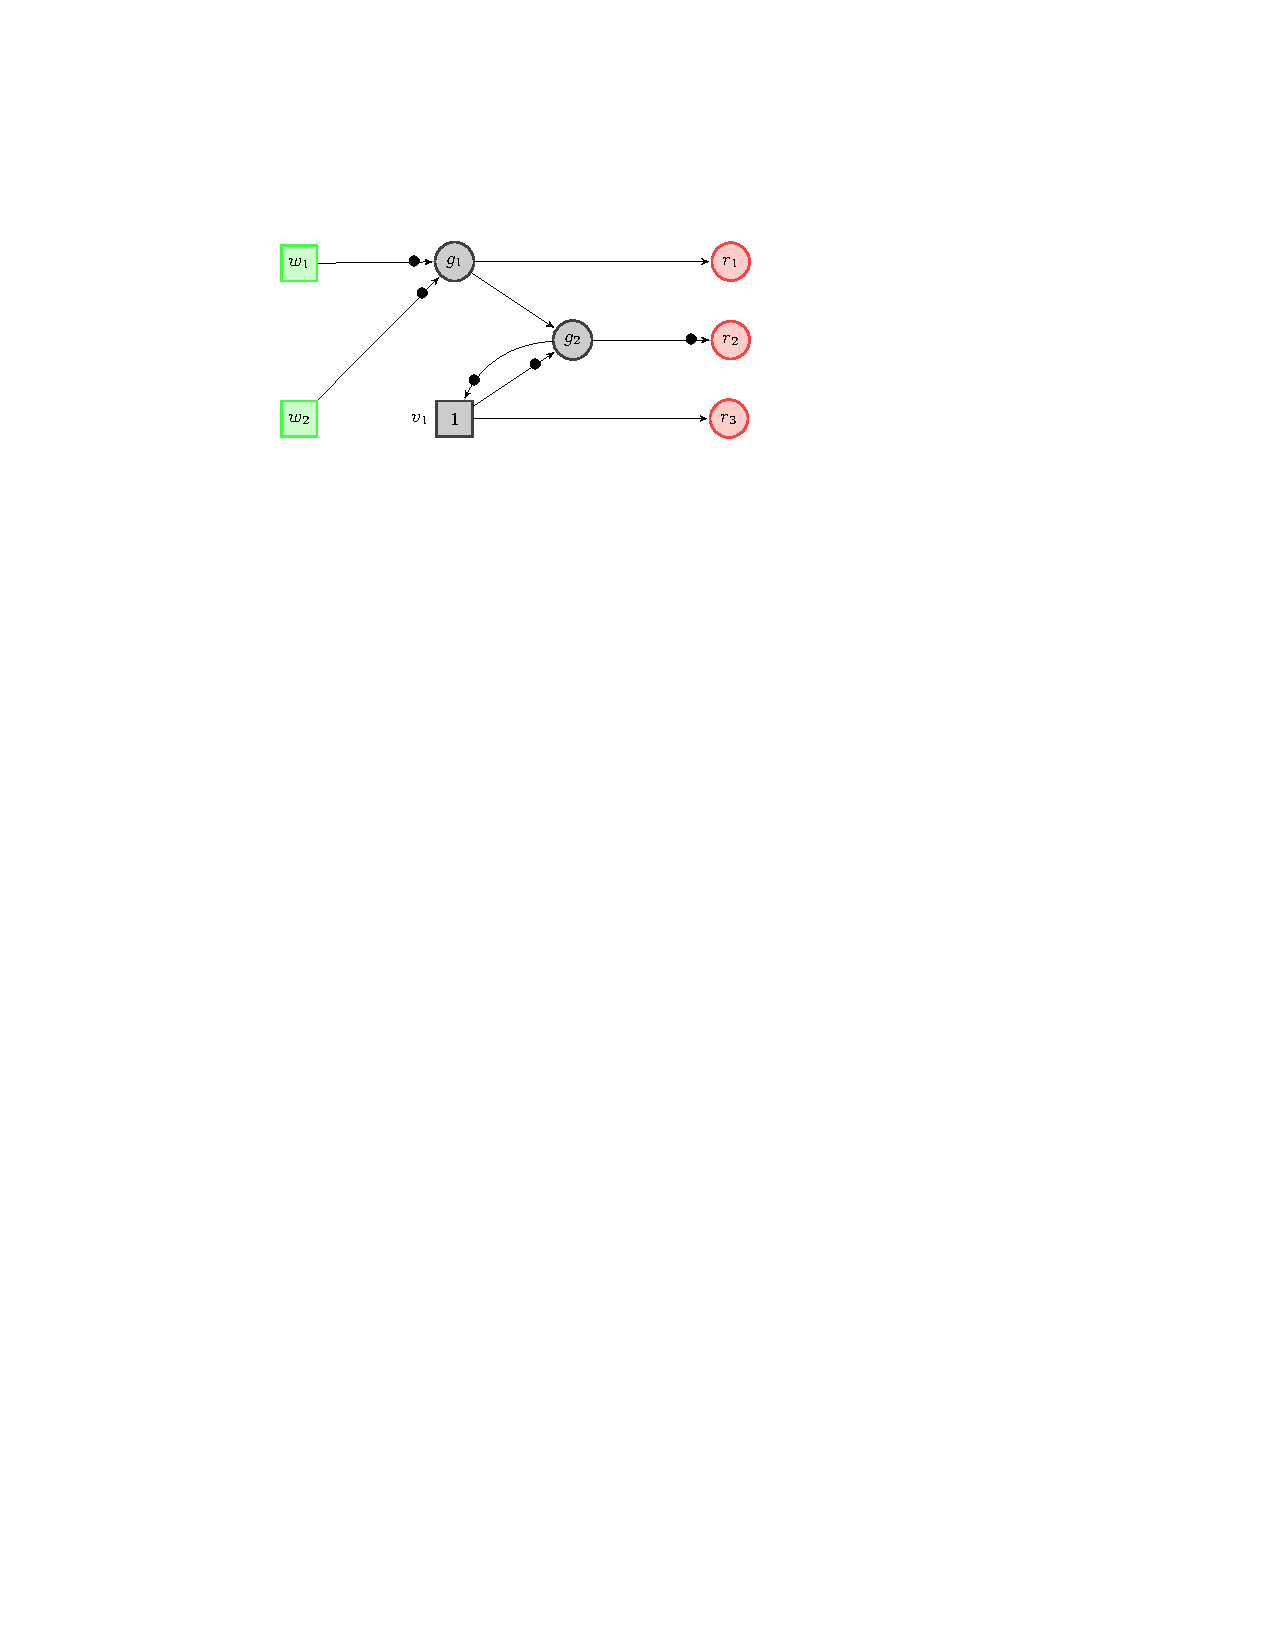
\includegraphics[width=\textwidth]{Example.pdf}
% \end{framed}
% \caption{\textbf{Left:} And-inverter graph describing a system with two
% inputs $w_1$ and $w_2$ (green boxes), one latch $v_1$ with initial value 1 (grey box), two gates $g_1$ and $g_2$ (gray circles), and three invariant requirements $r_1=\Always g_1$, $r_2=\Always \lnot g_2$ and $r_3=\Always v_1$ (red circles). 
% The arrows represent logical dependencies, and bullets in the arrows imply negation.}
% \label{fig:Preliminaries:AIGExample}
% \end{figure}
    %



\begin{figure}[!t]
	\begin{minipage}{0.6\textwidth}
	\begin{framed}
	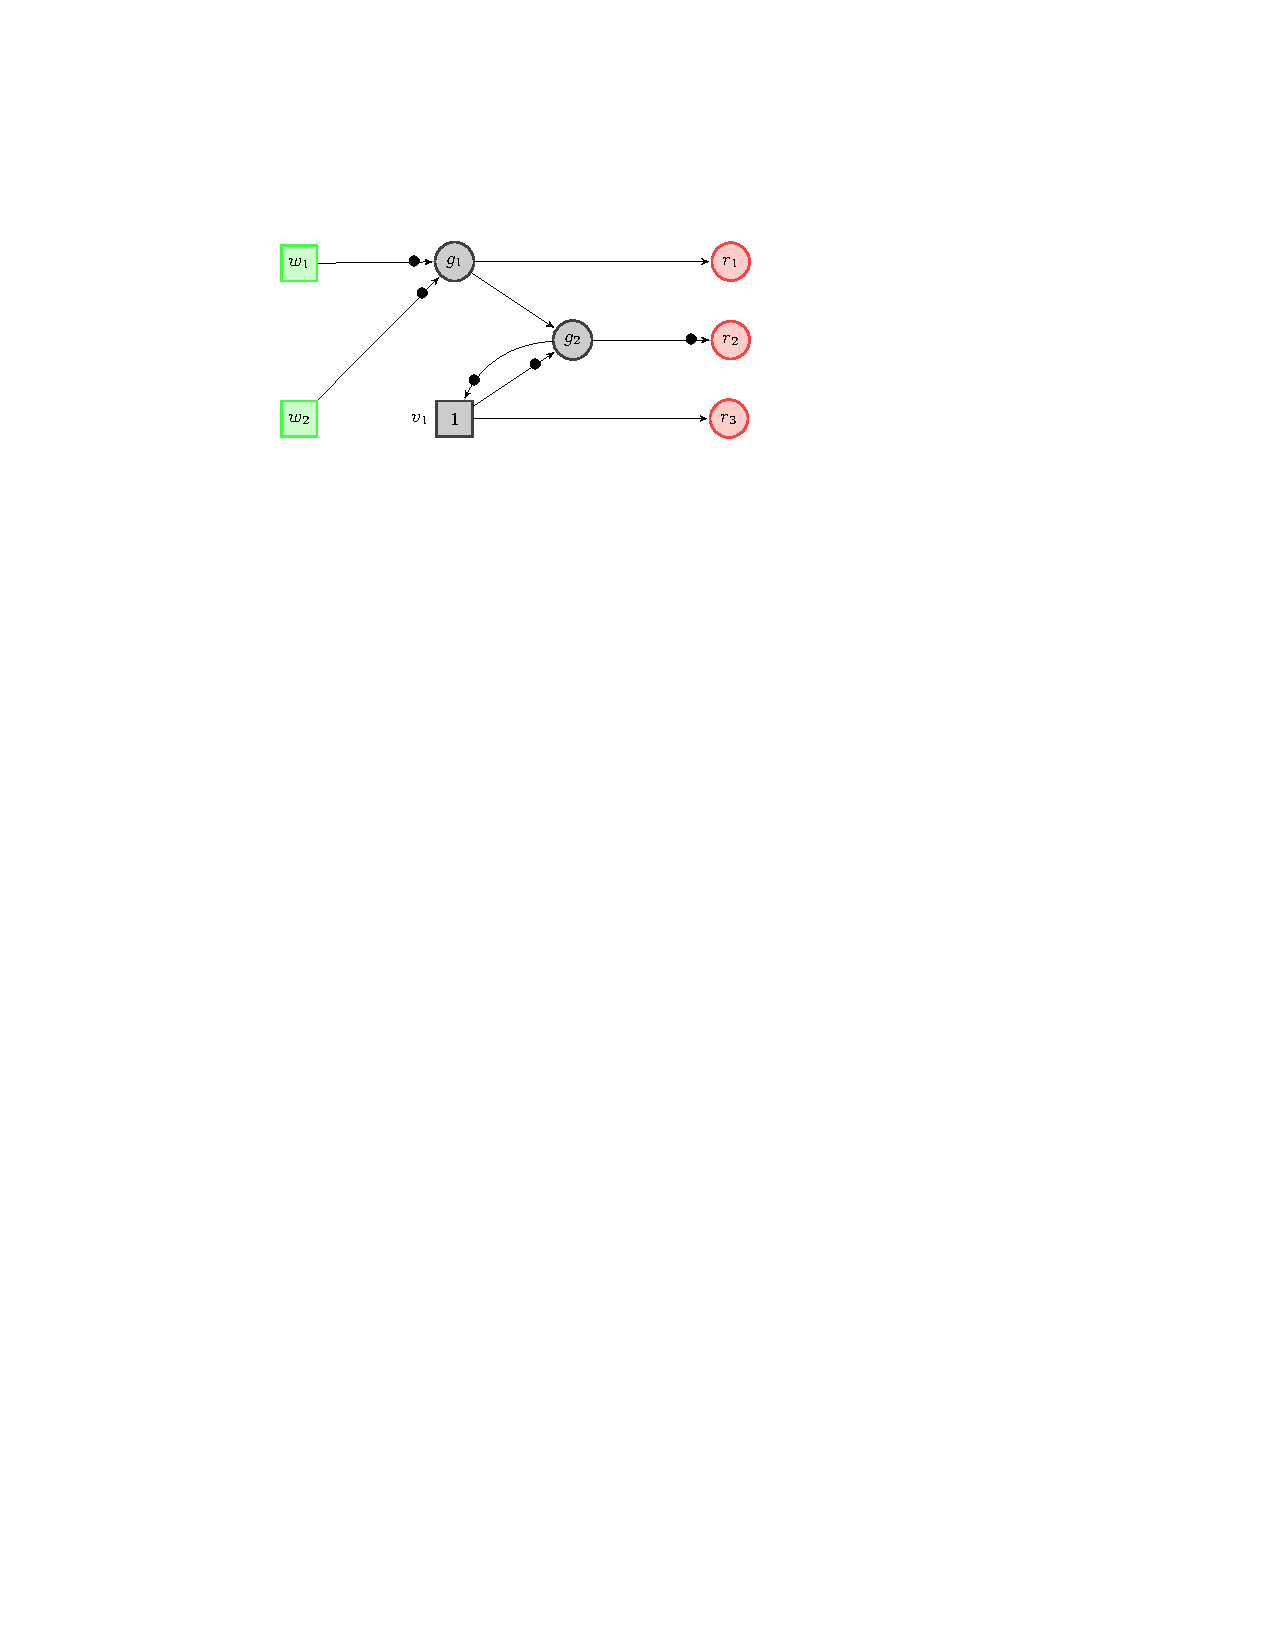
\includegraphics[width=\textwidth]{Example.pdf}
	\end{framed}
	\end{minipage}
	\begin{minipage}{0.35\textwidth}
	\centering
	\begin{framed}
	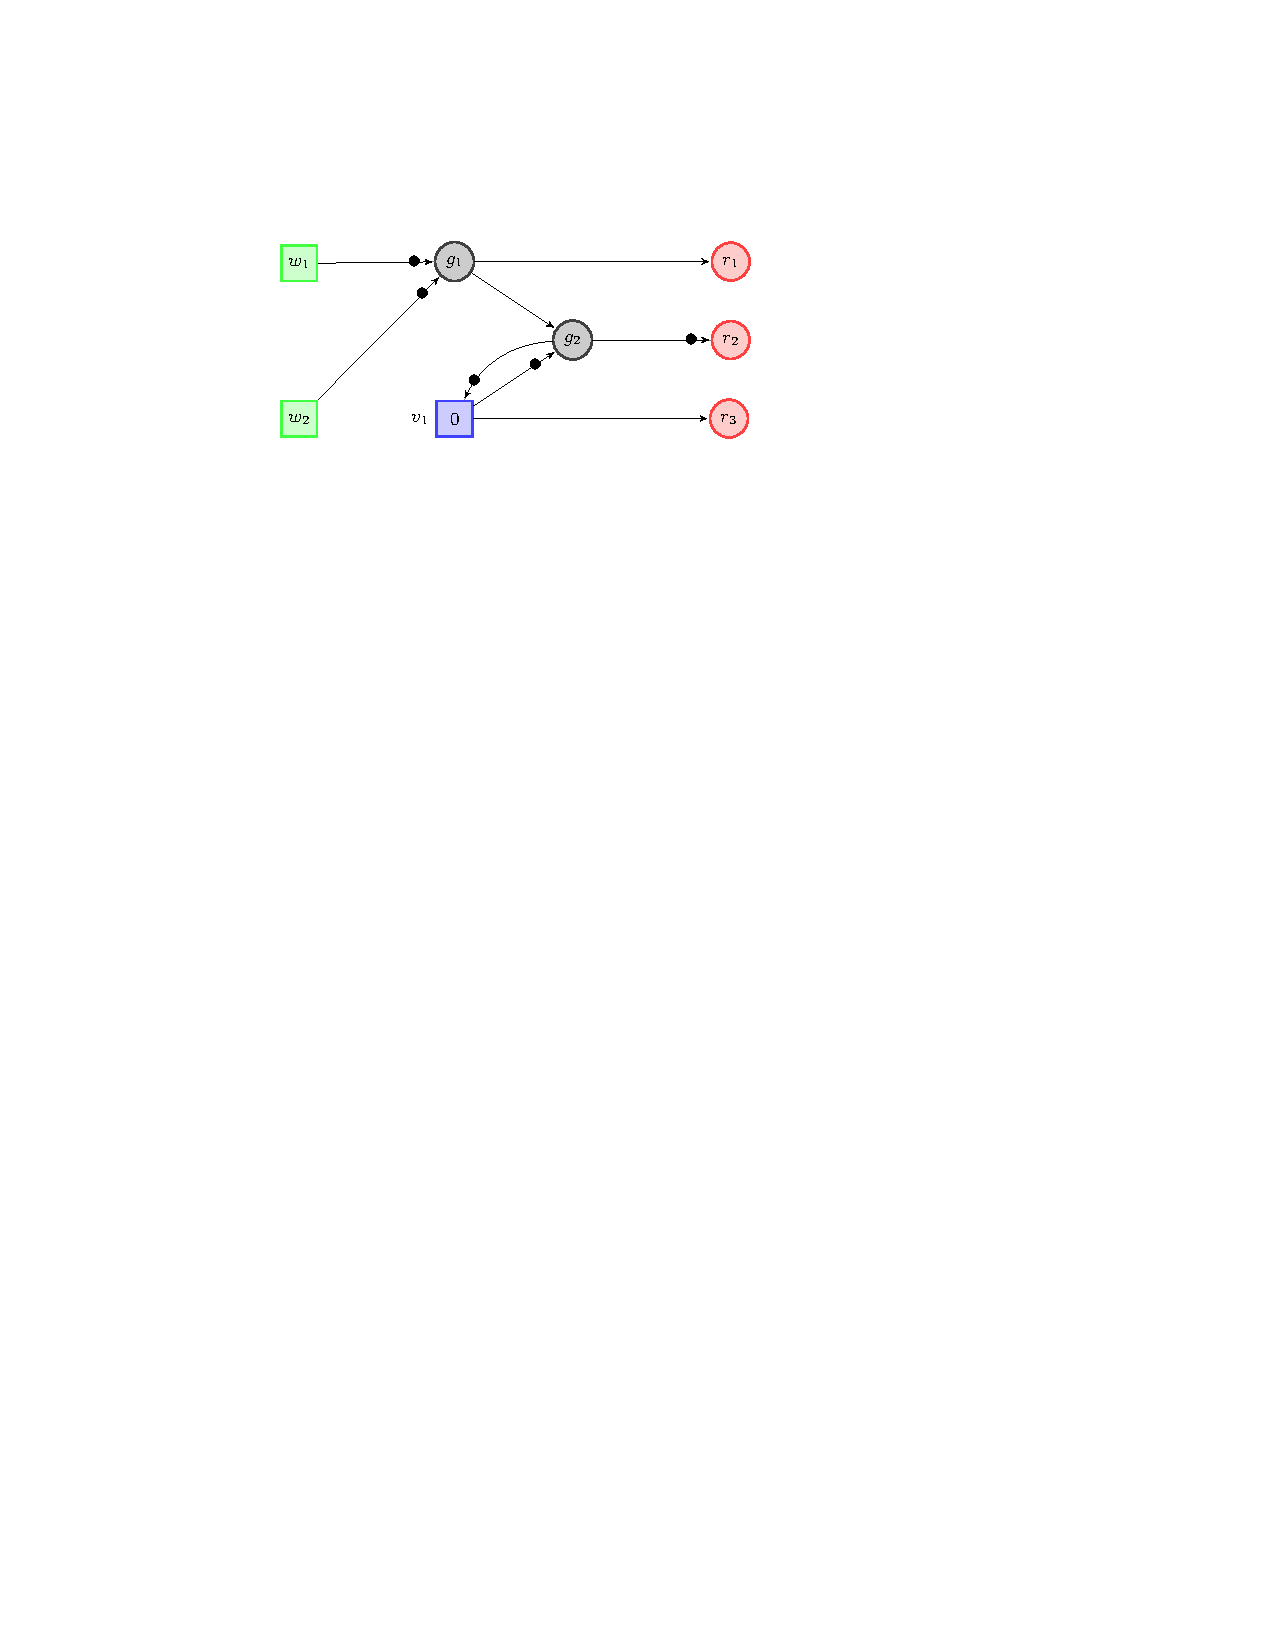
\includegraphics[width=\textwidth]{Attack2.pdf}\\
	\end{framed}
	\begin{framed}
	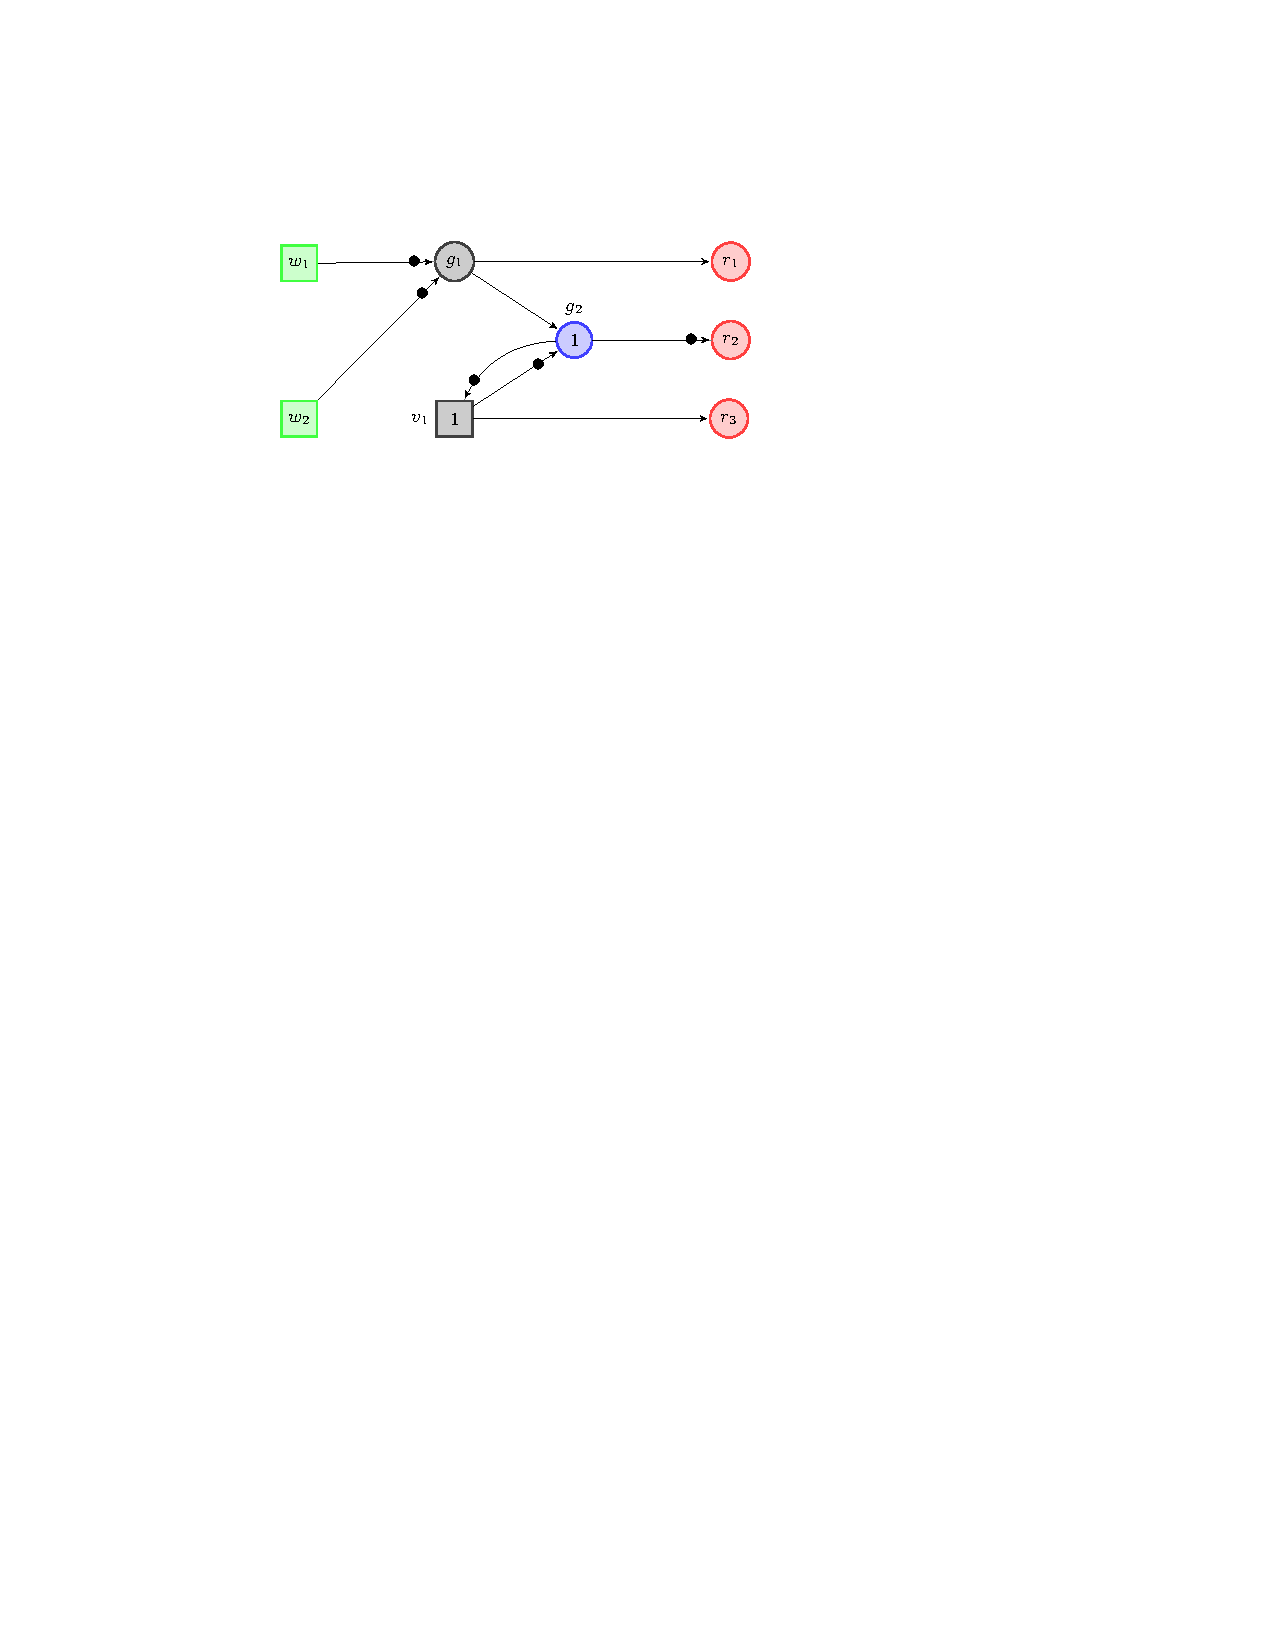
\includegraphics[width=\textwidth]{Attack1.pdf}
	\end{framed}
	\end{minipage}
	\caption{\textbf{Left:} An AIG with two
	inputs $w_1$ and $w_2$ (green boxes), one latch $v_1$ with initial value 1 (grey box), two gates $g_1$ and $g_2$ (gray circles), and three invariant requirements $r_1=\Always g_1$, $r_2=\Always \lnot g_2$ and $r_3=\Always v_1$ (red circles). 
	The arrows represent logical dependencies, and bullets in the arrows imply negation.
	\textbf{Right above}: an attacker that controls latch $v_1$ can set its initial value to 0 to break $r_2$ and $r_3$ in 0 steps. This attacker uses a spatial transformation to implement this attack.
	\textbf{Right below}: an attacker that controls gate $g_2$ can set its value to 1 at time 0 to break $r_2$ in 0 steps and $r_3$ in 1 step, because the value of $v_1$ at time 1 is 0. This attacker uses a dynamics transformation, since gates are not part of the state of AIGs.}%. An arrow with $!$ means negation}
	\label{fig:Classification:Example}
	\end{figure}

% In this section, we provide a motivational example of the problem of model checking compromised systems, and we illustrate how to classify attackers given a list of security requirements. 
 assume that an attacker $A$ controls the gate $g_2$ of the AIG shown on the left of Figure~\ref{fig:Classification:Example}. By controlling $g_2$, we mean that $A$ can choose the value of $g_2(t)$ at will for $t\geq 0$.This system fails $r_1$ at time $t$ if $w_1(t)=1$, so the attacker $A$ does not need to do anything to cause the system to fail $r_1$. Now, it is possible for $A$ to break $r_2$ at time $t=0$ and to break $r_3$ at time $t=1$ by setting $g_2(0)$ to $1$ via an attack, since $r_2=\Always \lnot g_2$, and by causing $v_1(1)$ to be equal to $0$. This attack breaks both requirements $r_2$ and $r_3$, but in general an attacker may need one attack to break one requirement, and a different attack to break another. We say that $A$ has the \emph{power to break the requirements} $r_1$, $r_2$ and $r_3$, since there are attacks in the capabilities of $A$ that break those requirements. Now, consider a different attacker $B$ which only controls the gate $g_1$. No matter what value $B$ chooses for $g_1(t)$ for all $t$, it is impossible for $B$ to break $r_2$ or $r_3$, so we say that $B$ only has the power to break $r_1$. 



If we allow attackers to control any number of coordinates, then there are $8$ different attackers, described by the subsets of $\set{v_1,g_1,g_2}$. We do not consider attackers that control inputs, because the model checking of invariant properties requires the property to hold for all inputs, so giving control of inputs to an attacker does not make it more powerful (i.e. the attacker cannot break more requirements than it already could without the inputs). Figure~\ref{fig:Classification:borders} illustrates the classification of attackers depending on whether they break a given requirement or not. Based on it, we can provide the following security guarantees: 1) the system cannot enforce $r_1$, and 2) that the system can only enforce $r_2$ and $r_3$ in the presence of attackers that are as capable to interact with the system as $\set{g_1}$ (i.e. they only control $g_1$ or nothing).

According to the classification, attacker $\set{g_2}$ is as powerful as the attacker $\set{v_1,g_1,g_2}$, since both attackers break the same requirements $r_1$, $r_2$ and $r_3$. This information may be useful to the designer of the system, because they may prioritise attackers that control less coordinates but are as powerful as attackers that control more when deploying defensive mechanisms.


\section{AIGs as $F$-coalgebras}
\label{sec:Classification:LatentBehaviours}
If we go by the strict definition of AIGs (see Section~\ref{sec:Preliminaries:AIGStates}), then only latches are part of the states of AIGs; inputs and gates are external. We, however, include gates into the state. Consider an AIG whose set of latches is $V$, its set of gates is $G$, its set of inputs is $W$ and its set of requirements is ${R}$. For each latch $v\in V$ there is an associated expression $v(t+1)$, for each gate $g\in G$, there is an associated expression $g(t)$, and each requirement $r\in {R}$ is of the form $r=\Always e$, where $e$ is an expression. 
Let $\vec{G}=2^G$, $\vec{V}=2^{V}$, $\vec{W}=2^W$ and let $\vec{{R}}=2^{{R}}$; we plan to use the set $\vec{V}\times \vec{G}$ as the carrier so that a state $(\vec{v},\vec{g})$ models the values for $\vec{v}(t+1)$ and $\vec{g}(t)$% (the values of $\vec{g}(0)$ depend on the input $\vec{w}(0)$)
. We now define the functor $F(X)=\vec{{R}}^{\vec{W}}\times X^{\vec{W}}$, and we define the $F$-coalgebra $(\vec{V}\times\vec{G},(\theta,\delta))$ where $(\theta,\delta)$ is a pair function with $\theta\colon \vec{V}\times \vec{G}\rightarrow \vec{{R}}^{\vec{W}}$, and $\delta\colon\vec{V}\times \vec{G} \rightarrow (\vec{V}\times \vec{G})^{\vec{W}}$. Given an input $\vec{w}\in \vec{W}$, the function $\delta$ maps the state $(\vec{v},\vec{g})$ to the state $(\vec{v}^{\vec{w}}, \vec{g}^{\vec{w}})$, which is defined for all $v'\in V$, $g'\in G$ and $w'\in W$, by 
\begin{align}
	\vec{v}^{\vec{w}}[v']&\triangleq \TheBehaviourOf{v'(t+1)},\\
	\vec{g}^{\vec{w}}[g']&\triangleq \TheBehaviourOf{g'(t)},
\end{align}
where $\TheBehaviourOf{g(t)}$ is the result of evaluating the expression $g'(t)$ by assuming $w'(t)=\vec{w}[w']$ and $v'(t)=\vec{v}[v']$. Note that if the expression $g'(t)$ depend on the value of $g''(t)$ where $g''$ is another gate, then we assume $g''(t)=\vec{g}^{\vec{w}}[g'']$ (AIGs are acyclic in their dependencies, only looping back to latches). Similarly, $\TheBehaviourOf{v'(t+1)}$ is the result of evaluating the expression $v(t+1)$ by assuming $w'(t)=\vec{w}[w']$, $v'(t)=\vec{v}[v']$, and $g'(t)=\vec{g}^{\vec{w}}[g']$. % instead of $g'(t)=\vec{g}[g']$. 

% for $v''\in V$, $w'\in W$ and $g''\in G$. 
The function $\theta$ evaluates the requirements given an input $\vec{w}$; for $r \in {R}$, we define
\begin{align}
	\theta(\vec{v},\vec{g})(\vec{w})[r]\triangleq \TheBehaviourOf{e(t)}, \quad \text{ if $r=\Always{e}$}, 
\end{align}
where $\TheBehaviourOf{e(t)}$ is the result of evaluating the expression $e(t)$ by assuming $w'(t)=\vec{w}[w']$, $v'(t)=\vec{v}[v']$ and $g'(t)=\vec{g}^{\vec{w}}[g']$.

%Since the set $\vec{V}\times \vec{G}$ is the carrier, 
In the following we show how to use bounded model checking to find spatial transformations which reveal a latent coalgebra that fails one or more security requirements. %whose coordinates are $V\cup G$, 
% Since the carrier is the set $\vec{V}$, spatial transformations do not directly transform the state of gates. If an attacker wants to affect a gate, they must do so via transitive data dependencies. More precisely, if a gate $g$ depends on a latch $v$ (e.g. $g(t)=v(t) \land \lnot k(t)$ where $k$ is some component, then an attacker controlling $v$ might affect $g$ by manipulating the value of the state at coordinate $v$. If the value of a gate $g$ does not transitively depend on any latch (e.g., $g_1$ in Figure~\ref{fig:Classification:Example}), then $g$ must only depend on inputs. %This follows the ideology of latent behaviour analysis, where we purposely restrict attackers to affect the state of the system.

% 



%------------------------------------------------------------------------------------------------------------------------------------------------

%-------------------------------------------------------------------------------------------------------------------------------------------------
\section{Bounded Model Checking of in the Presence of Attackers}
\label{sec:bmc}
% We recall the research questions that motivate this work: \textbf{RQ1)} given a system and a list of security requirements, how do we systematically generate attackers that can potentially break these requirements, and how do we verify if they are successful? and \textbf{RQ2)} which techniques can help us \emph{classify} attackers, i.e., to map each attacker to the set of requirements that it breaks? 
In this section, we %aim to answer these research questions on a theoretical level by 
formalise the problem of attacker model classification for AIGs using bounded model checking in the presence of attackers. More precisely, %to answer \textbf{RQ1},
we formalise attackers and their interactions with systems, and we show how to systematically generate bounded model checking problems that determine whether some given attacker breaks the security requirement being checked. We then propose two methods for the classification of attackers: 1) a brute-force method that creates a model checking problem for each attacker-requirement pair, and 2) a method that incrementally empowers attackers to find \emph{minimal attackers}, i.e. attackers which represent large portions of the universe of attackers thanks to a monotonicity relation between the set of coordinates controlled by the attacker and the set of requirements that the attacker breaks. %The latter method is a theoretical approach to answer \textbf{RQ2}, while its practical usefulness is evaluated in Section~\ref{sec:evaluation}.

\subsection{Attackers and Compromised Systems}
We modify the equations that are associated to the coordinates controlled the attacker to incorporate the possible actions of such attacker into an AIG. Formally, let $S=(W,V,G)$ be a system described by an AIG, let $R=\set{r_1, \ldots, r_n}$ be a set of invariant requirements for $S$, and let $C=V\cup G$ be the set of coordinates of $S$. An \emph{attacker model} $A$ is any subset of $C$. We refer to attackers fitting the model $A$ as \emph{$A$-attackers}. If a coordinate $c$ belongs to an attacker model $A$, then an $A$-attacker has the \emph{capability to interact with $S$ through} $c$. To capture this interaction, we modify the equations of every latch $v\in V$ to be parametrised by an attacker model $A$ as follows: the original transition equation $v(t+1)=e(t)$ and the initial equation $v(0)=b$ change to
\begin{align}
\label{eq:badLatch}
v(t+1) = \begin{cases}
e(t), \quad &\text{if $v\not \in A$;}\\
A_v(t+1), \quad &\text{otherwise},
\end{cases}
\quad 
v(0)= \begin{cases}
b, \quad &\text{if $v \not \in A$;}\\
A_v(0), \quad &\text{otherwise.}
\end{cases}
\end{align}
where $A_v(t)$ is a value chosen by an $A$-attacker at time $t$. Similarly, we modify the equation of gate $g\in G$ as follows: the original equation $g(t)=e_1(t)\land e_2(t)$ changes to
\begin{align}
\label{eq:badGate}
g(t) = \begin{cases}
e_1(t)\land e_2(t), \quad &\text{if $g\not \in A$;}\\
A_g(t), \quad &\text{otherwise},
\end{cases}
\end{align}
where $A_g(t)$ is, again, a value chosen by an $A$-attacker at time $t$. We use $A[S]$ to denote the system $S$ under the influence of an $A$-attacker; i.e., $A[S]$ is the modified system of equations. 

We now apply the definition of attacks as state transformations. An \emph{attack from an $A$-attacker}, is a function $m\colon \vec{G}\times \vec{V}\rightarrow \vec{G}\times \vec{V}$ that assigns a value to each coordinate in $A$. Given a state $\vec{x}\in \vec{G}\times \vec{V}$ and an attack $m\colon \vec{G}\times \vec{V}\rightarrow \vec{G}\times \vec{V}$, we define the \emph{ effect of $m$ on coordinates $A$ at state $\vec{x}$}, denoted $m(\vec{x})|_A\colon A\rightarrow 2$, by
\begin{align}
	m(\vec{x})|_{A}[a]\triangleq m(\vec{x})[a].
\end{align}
In the following, we consider a strategy to build an attacks for an $A$-attacker by computing the effects on coordinates $A$ in the context given by the initial state of the AIG and its successor states. Formally, we propose finding a finite sequence of vectors $\vect{a}_0,  \ldots, \vect{a}_t$ such that the vectors fix the values of all $A_c(k)$ by assuming $A_c(k)=\vect{a}_k(c)$, with $c\in A$ and $0 \leq k \leq t$. In this sense, the sequence $(\vect{a}_0, \ldots, \vect{a}_t)$ models an \emph{attack strategy to break requirements}.

% An \emph{attack strategy} is a finite sequence of attacks $(\vect{a}_0, \vect{a}_1, \ldots, \vect{a}_t)$ that fixes the values of all $A_c(k)$ (used in the equations above) by $A_c(k)=\vect{a}_k(c)$, with $c\in A$ and $0 \leq k \leq t$. %Since we have changed the semantics of the system, it is possible that $A[S]$ only satisfies a subset of requirements in $R$. 
\begin{definition}[Broken Requirement]
\label{def:brokenRequirement}
Given a requirement $r\in R$ with $r=\Always e$, we say that an $A$-attacker \emph{breaks the requirement $r$ (at time $t$)} if and only if there exists a sequence of inputs $\vec{w}_0, \ldots, \vec{w}_t$ and an attack strategy $\vect{a}_0, \ldots, \vect{a}_t$ such that $e(t)$ is false if we assume $w'(k)=\vec{w}_k[w']$ and $a'(k)=\vec{a}_k[a']$, with $0\leq k\leq t$, $w'\in W$, and $a'\in A$. We denote the set of requirements that an $A$-attacker breaks by $A[R]$. 
\end{definition}

We now define two partial orders for attackers: \textbf{1)} an $A_i$-attacker is strictly less \emph{capable} (to interact with the system) than an $A_j$-attacker in the 
context of $S$ %, denoted $A_i \leq A_j$ 
iff $A_i\subseteq A_j$ and $A_i \neq A_j$. An {$A_i$-attacker is equally capable to an $A_j$-attacker iff $A_i= A_j$}; and \textbf{2)} an $A_i$-attacker is strictly less \emph{powerful} than an $A_j$-attacker in the 
context of $S$ and $R$ %, denoted $A_i \leq A_j$ 
iff $A_i[R]\subseteq A_j[R]$ and $A_i[R]\neq A_j[R]$. Similarly, {$A_i$-attacker is equally powerful to an $A_j$-attacker iff $A_i[R]= A_j[R]$}. %We simply state that $A_i$ is less capable than $A_j$ if $S$ is clear from the context. 
% We simply say that $A_i$ is less powerful than $A_j$ if $S$ and $R$ are clear from the context.

%\subsection{Model Checking in the Presence of Attackers}
We can now properly present the problem of \emph{attacker model classification}.
\begin{definition} [Attacker Classification via Verification]
\label{def:AttackerQuantification}
Given a system $S$, a set of requirements $R$, and a set of $h$ attacker models
$\set{A_1, \ldots , A_h}$, for every attacker model $A$, we compute the set $A[R]$ of requirements that an $A$-attacker breaks by performing model checking of each requirement in $R$ on the compromised system $A[S]$. 
\end{definition}

%The duality between attackers and sets of coordinates enables the following assertions: a set of coordinates $B$ is \emph{safe} if and only if we can prove that attacker $B$ cannot break any requirements, i.e., $B[R]=\emptyset$; otherwise, the set of coordinates $B$ is  \emph{vulnerable}. 
Definition~\ref{def:AttackerQuantification} assumes that exhaustive verification is possible for $S$ and the compromised versions $A[S]$ for all attackers $A$. However, if exhaustive verification is not possible (e.g., due to time limitations or memory restrictions), we consider an alternative formulation using \emph{bounded model checking} (BMC): 
\begin{definition} [Attacker Model Classification using BMC]
\label{def:BoundedModelCheckingOfSystems}
Let $S$ be a system, $R$ be a set of requirements, and $t$ be a natural number. Given a set of attacker models $\set{A_1, \ldots , A_h}$, for each attacker model $A$ , we compute the set $A[R]$ of requirements that an $A$-attacker breaks \emph{using a strategy of length up to $t$} on the compromised system $A[S]$. 
\end{definition}
In the following, we show how to construct a SAT formula that describes the attacker model classification problem using BMC. 

\subsection{A SAT Formula for BMC up to $t$ Steps}
For a requirement $r=\Always e$ and a time step $t\geq 0$, we are interested in finding an attack strategy that causes the value of $e(k)$ to be false for some $k$ with $0\leq k \leq t$. To capture this notion, we define the proposition $\mathtt{goal}(r,t)$ by
\begin{align}
\mathtt{goal}(\Always e,t) \triangleq \bigvee_{k=0}^t{\lnot e(k)}.
\end{align}
We inform the SAT solver of the equalities and dependencies between expressions given by the definition of the AIG (e.g., that $e(k) \Leftrightarrow \lnot v_1(k)$). Inspired by the work of Biere \emph{et al.} \cite{BMCWithoutBDDs}, we transform the equations into a Conjunctive Normal Form formula (CNF) that the SAT solver can work with using  \emph{Tseitin encoding} \cite{TseitinEncoding}. Each equation of the form 
\begin{align*}
&v(0)= \begin{cases}
b, \quad &\text{if $v \not \in A$;}\\
A_v(0), \quad &\text{otherwise,}
\end{cases}
\end{align*}
becomes the formula of the form
\begin{align}
{\left(v^{\downarrow} \lor (v(0) \Leftrightarrow b ) \right)\land \left(\lnot v^{\downarrow} \lor (v(0) \Leftrightarrow A_v(0)) \right)},
\end{align}
where $v^{\downarrow}$ is a literal that marks whether the latch $v$ is an element of the attacker model $A$ currently being checked; i.e., we assume that $v^{\downarrow}$ is true if $v\in A$, and we assume that $v^{\downarrow}$ is false if $v\not \in A$. Consequently, if $v\not \in A$, then $v(0) \Leftrightarrow b$ must be true, and if $v \in A$, then $v(0)  \Leftrightarrow A_v(0) $ must be true. We denote this proposition by $\mathtt{encode}(v,0)$, and it informs the SAT solver about the initial state of the AIG.
 
Similarly, for $0\leq k<t$, each equation of the form 
\begin{align*}
&v(k+1) = \begin{cases}
e(k), \quad &\text{if $v\not \in A$;}\\
A_v(k+1), \quad &\text{otherwise},
\end{cases}\quad
\end{align*}
translates to a formula of the form
\begin{align}
&\left(v^{\downarrow} \lor (v(k+1) \Leftrightarrow e(k) ) \right)\land \left(\lnot v^{\downarrow} \lor (v(k+1) \Leftrightarrow A_v(k+1)) \right).
\end{align}
We call this formula $\mathtt{encode}(v,k)$. %We now use the Tseitin encoding of $p \Leftrightarrow (q \land r)$, i.e., $(p \lor \lnot q \lor \lnot r)\land (\lnot p \lor q)\land  (\lnot p \lor r)$, to encode gates. 

Finally, for $0\leq k \leq t$, each equation of the form
\begin{align*}
&g(k) = \begin{cases}
e_1(k)\land e_2(k), \quad &\text{if $g\not \in A$;}\\
A_g(k), \quad &\text{otherwise},
\end{cases}
\end{align*}
becomes a formula of the form
\begin{align}
&\left(g^{\downarrow} \lor (g(k) \Leftrightarrow e_1(k)\land e_2(k) ) \right)\land \left(\lnot g^{\downarrow} \lor (g(k) \Leftrightarrow A_g(k)) \right),
\end{align}
where $g^{\downarrow}$ is a literal that marks whether the gate $g$ is an element of the attacker model $A$ currently being checked in a similar way that the literal $v^\downarrow$ works for the latch $v$. We refer to this formula by $\mathtt{encode}(g,k)$.
%Consider a coordinate $c$ and an attacker $A$. Under the new system of equations, if $c\in A$, then we assume $c^{\downarrow}$ and the value of coordinate $c$ at time $k$ depends only on the literal $A_c(k)$; if $c\not\in A$, then we assume $\lnot c^{\downarrow}$ and we use the original semantics of the system to determine the value of $c$. 


Given an attacker model $A$, to perform SAT solving, we need to find an assignment of inputs in $W$ and attacker actions for each coordinate $c$ in $A$ over $t$ steps, i.e., an assignment of ${|W\times A|\times t}$ literals. The SAT problem for checking whether requirement $r$ is safe up to $t$ steps, denoted $\mathtt{check}(r,t)$, is defined by 
\begin{align}
\label{eq:naiveCheck}
\mathtt{check}(r,t)\triangleq\mathtt{goal}(r,t)\land\! \bigwedge_{c\in (V \cup G)}\left( \bigwedge_{k=0}^{t}{\mathtt{encode}(c,k)}\right).
\end{align}
If the SAT solver can provide an assignment of literals which satisfy $\mathtt{check}(r,t)$, then an $A$-attacker breaks the requirement $r$.
\begin{proposition}
\label{prop:Correctness}
For a given attacker model $A$ and a requirement $r=\Always e$, if we assume the literal $c^{\downarrow}$ for all $c \in A$ and we assume $\lnot x^{\downarrow}$ for all $x\not\in A$ (i.e., $x\in (V \cup G)-A$), then an $A$-attacker breaks the requirement $r$ in $t$ steps (or less) if and only if $\mathtt{check}(r,t)$ is satisfiable.
\end{proposition}

\begin{proof}
We first show that if an $A$-attacker breaks the requirement in $t$ steps or less, then $\mathtt{check}(r,t)$ is satisfiable. Since an $A$-attacker breaks $r=\Always e$ in $t$ steps or less, then, by Definition~\ref{def:brokenRequirement}, there exists an assignment of inputs $(\vect{w}_0, \ldots, \vect{w}_k)$ and an attacker strategy $(\vect{a}_0, \ldots, \vect{a}_k)$ which causes $e(k)$ to be false for some $k\leq t$; this means that $\mathtt{goal}(r,t)$ is satisfiable, which, in turn, makes $\mathtt{check}(r,t)$ satisfiable.

We now show that if $\mathtt{check}(r,t)$ is satisfiable, then an $A$-attacker breaks the requirement $r$ in $t$ or less steps. If $\mathtt{check}(r,t)$ is satisfiable then $\mathtt{goal}(r,t)$ is satisfiable, and $e(k)$ is false for some $k\leq t$. Consequently, there is an assignment of inputs $\vect{w}(k)$ and attacker actions $A_c(k)$, such that the $\mathtt{encode}(c,k)$ formulae are satisfied for all $c\in A$. By assuming $\vect{a}_k(c)=A_c(k)$ and $\vect{w}_k =\vect{w}(k)$, we obtain a witness input sequence and a witness attack strategy which proves that an $A$-attacker breaks $r$ in $k$ steps (i.e., in $t$ steps or less since $k\leq t$).
\end{proof}

Algorithm~\ref{alg:BadQuantification} describes a naive strategy to compute the sets $A[R]_t$ for each attacker model $A$; i.e. the set of requirements that an $A$-attacker breaks in $t$ steps (or less). Algorithm~\ref{alg:BadQuantification} works by solving, for each of the $2^{|V \cup G|}$ different attacker models, a set of $|R|$ SAT problems, 
{
each of which has a size of at least $\mathcal{O}\left({|W\cup V\cup G|\times t}\right)$ on the worst case.}

\begin{figure}[!t]
\centering
{
%\begin{framed}
\begin{algorithm}[H]
 \KwData{system $S=(W,V,G)$, a time step $t\geq 0$, a set of requirements $R$.}
 \KwResult{A map that maps the attacker $A$ to $A[R]_t$.}
Map $\mathcal{H}$\;
\For{\!\!\textbf{each} $r \in R$}
{
\For{\!\!\textbf{each} $A$ such that $A \subseteq (V\cup G)$}
	{
		\If{$\mathtt{check}(r,t)$ is satisfiable while assuming $c^\downarrow$ for all $c\in A$}
		{
			insert $r$ in $\mathcal{H}(A)$\;
		}
	 }
}
 \Return $\mathcal{H}$\;
 \caption{Naive attacker model classification algorithm.}
 \label{alg:BadQuantification}
\end{algorithm}
%\end{framed}
}
\end{figure}

We now propose two sound heuristics in an attempt to improve Algorithm~\ref{alg:BadQuantification}: the first technique aims to reduce the size of the SAT formula, while the other heuristic aims to record and propagate the results of previous verifications among the set of attacker models so that some calls to the SAT solver are avoided.

\subsection{Heuristics: Isolation and Monotonicity}
\emph{Isolation} is a strategy that uses data dependency analysis to prove that is impossible for a given attacker model to break some requirement. Informally, a requirement $r$ is isolated from an attacker model $A$ if no flow of information can occur from the coordinates in $A$ to the expression that defines $r$. To formally capture isolation, we first extend the notion of IOC to attacker models. The \emph{IOC of an attacker model $A$}, denoted $\blacktriangle(A)$, is defined by the union of IOCs of the coordinates in $A$; more precisely, 
\begin{align}
	\blacktriangle(A) \triangleq \bigcup\set{\blacktriangle(c)|c \in A}.
\end{align}
Isolation happens whenever the IOC of $A$ is disjoint from the COI of $r$, implying that $A$ cannot interact with $r$.
\begin{proposition}[Isolation]
\label{theo:isolation}
Let $A$ be an attacker model and $r$ be a requirement that is satisfied by the AIG. If $\blacktriangle(A)\cap \blacktriangledown(r)=\emptyset$, then an $A$-attacker does not break $r$.\end{proposition}
\begin{proof}

For an $A$-attacker to break the requirement $r$, there must be a coordinate $c \in \blacktriangledown(r)$ whose behaviour is affected by the presence of such $A$-attacker, causing $r$ to fail. In such a case, there must be a dependency between the variables directly controlled by the $A$-attacker and $c$, since $A$-attackers only choose actions over the coordinates they control; implying that $c\in \blacktriangle(A)$. This contradicts the premise that the IOC of $A$ and the COI of $r$ are disjoint, so the coordinate $c$ cannot exist. \qed
\end{proof}

Isolation reduces the SAT formula by dismissing attacker models that are outside the COI of the requirement to be verified. Isolation works similarly to \emph{COI reduction} (see \cite{ToSplitOrToGroup,GraphLabelingForEfficientCOIComputation,HandbookOfSatisfiability,HandbookOfModelChecking,OptimizedModelCheckingOfMultipleProperties}), and it transforms Equation \ref{eq:naiveCheck} into
\begin{align}
\label{eq:isolation}
\mathtt{check}(r,t)\triangleq\mathtt{goal}(r,t)\land\! \bigwedge_{c\in (\blacktriangledown(r)- W)}\left( \bigwedge_{k=0}^{t}{\mathtt{encode}(c,k)}\right)
\end{align}

\emph{Monotonicity} is a strategy that uses the following relation between capabilities and power of attacker models: if an attacker model $B$ has at least the same capabilities as an attacker model $A$ (i.e. $A\subseteq B$), then anything that an $A$-attacker can do, a $B$-attacker can do as well.
\begin{proposition}[Monotonicity]
\label{theo:monotonicity}
For attacker models $A$ and $B$ and a set of requirements $R$, if $A\subseteq B$, then $A[R]\subseteq B[R]$.
\end{proposition}
\begin{proof}
If $A\subseteq B$, then a $B$-attacker can always choose the same attack strategies that an $A$-attacker uses to break the requirements in $A[R]$; however, there may be strategies that a $B$-attacker uses that an $A$-attacker cannot, e.g., if $B$ has a coordinate that $A$ does not. Consequently, $A[R]\subseteq B[R]$.
\end{proof}
We use monotonicity to define a notion of {minimal (successful) attacker model} for a requirement $r$: an attacker model $A$ is a \emph{minimal attacker model} for a requirement $r$ if and only if an $A$-attacker breaks $r$, and there is no attacker model $B\subset A$ such that a $B$-attacker breaks $r$. In the following sections, we describe a methodology for attacker model classification that focuses on the identification of these minimal attacker models. %We expand on this notion in the following sections.

\subsection{Minimal (Successful) Attacker Models}
By monotonicity, any attacker model that is more capable than a minimal attacker models for a requirement $r$ breaks $r$, and any attacker model that is less capable than a minimal attacker model for $r$ cannot break $r$; otherwise, this less capable attacker model would be a minimal attacker model. In this sense, the minimal attacker models for $r$ not only partition the set of attacker models into those that break $r$ and those who do not, they create a frontier in the lattice of attacker models. For example, on the left of Figure~\ref{fig:Classification:borders}, the minimal attacker models for requirement $r_2$ are $\set{v_1}$ and $\set{g_2}$; the frontier (shown by the red arrows) is formed because any attacker model that includes them also breaks $r_2$. For these reasons, we reduce the problem of attacker model classification to the problem of finding the minimal attacker models for all requirements.

\subsubsection{Existence of a Minimal Attacker.} A requirement $r$ that is isolated from an attacker model $A$ remains safe in the presence of an $A$-attacker. Thus, for each requirement $r\in R$, if an attacker model $A$ breaks $r$, then $A$ must be a subset of ${\blacktriangledown(r)-W}$. 
Out of all the attacker models that could break $r$, the most capable attacker model is $\blacktriangledown(r)-W$. For succinctness, we henceforth denote the attacker $\blacktriangledown(r)-W$ by $r^{max}$. We check the satisfiability of $\mathtt{check}(r,t)$ with respect to the attacker model $r^{max}$ to learn whether there {exists} any other attacker model that breaks $r$ in $t$ steps; if $\mathtt{check}(r,t)$ is not satisfied, then no attacker model breaks $r$, otherwise we contradict monotonicity.

\begin{corollary}
From monotonicity and isolation (cf. Propositions \ref{theo:monotonicity} and \ref{theo:isolation}), if attacker $r^{max}$ cannot break the requirement $r$, then there are no minimal attacker models for $r$. %Equivalently, if $r^{max}$-attacker models cannot break $r$, then $r$ does not belong to any set of broken requirements $A[R]$.
\end{corollary}
\begin{figure}[!h]
\centering
{
%\begin{framed}
\begin{algorithm}[H]
 \KwData{system $S$, a requirement $r$, and a time step $t\geq 0$. }
\KwResult{set $M$ of {minimal} attacker models for $r$, bounded by $t$.}
{
\If{$check(r,t)$ is \textbf{not} satisfiable while assuming $c^\downarrow$ for all $c\in r^{max}$}
	{	
		\Return $\emptyset$\;
	}
}
Set: $P=\set{\emptyset}$, $M= \emptyset$; \quad /\!/($P$ contains the empty attacker model $\emptyset$)\\
\While{$P$ is not empty}
{
	extract $A$ from $P$ such that $A$ is minimal with respect to set inclusion\;
	\If{\textbf{not} (exists $B \in M \text{ such that } B \subseteq A)$}
	{	
        	\eIf{$\mathtt{check}(r,t)$ is satisfiable when assuming $c^\downarrow$ for all $c\in A$}
        	{
        		insert $A$ in $M$\;
        	}
        	{
        		 \For{\!\!\textbf{each} $c \in (r^{max} - A)$}
        		 {
        			insert $A \cup \set{c}$ in $P$\;
        	 	}
        
        	}
	}
	
}
\Return $M$\;

 \caption{The $\mathtt{MinimalAttackerModels}$ algorithm.}
 \label{alg:CheckRequirement}
\end{algorithm}
%\end{framed}
}
\vspace{-0.5cm}
\end{figure}

%\paragraph{Finding Minimal Attacker models.} 
After having confirmed that at least one non-isolated attacker model breaks $r$, we focus on finding minimal attacker models. Our strategy consist of starting with the smallest possible sets of capabilities (i.e. non-isolated attacker models), and systematically increasing those sets of capabilities when they fail to break the requirement $r$; we continue increasing them until they do, or we find that they are a superset of a different minimal attacker model. Algorithm~\ref{alg:CheckRequirement} describes this empowering procedure to computes the set of minimal attacker models for a requirement $r$, which we call $\mathtt{MinimalAttackerModels}$. As mentioned, we first check to see if a minimal attacker model exists (Lines 1-3); then we start evaluating attacker models in an orderly fashion by always choosing the least capable attacker model in the set of pending attacker models $P$ (Lines 5-16). Line 7 uses monotonicity to discard the attacker model $A$ if there is a known successful attacker model $B$ with $B\subseteq A$. Line 8 checks if the attacker model $A$ breaks $r$ in $t$ steps (or less); if so, then $A$ is a minimal attacker model for $r$ and is included in $M$ (Line 9); otherwise, we empower $A$ with a new coordinate $c$, and we add these new attacker models to $P$ (Lines 11-13). We note that Line 11 relies on isolation, since we only add coordinates that belong to the COI of $r$.

\begin{example}
We recall the motivational example from Section~\ref{sec:Classification:Example}. 
Consider the computation of $\mathtt{MinimalAttackerModels}$ for requirement $r_2$. In this case, $r_2^{max}$ is $\set{g1,g2,v_1}$, which breaks $r_2$. The model $r_2^{max}$ confirms the existence of a minimal non-isolated attacker model (Lines 1-3). We start to look for minimal attacker models by checking the attacker model $\emptyset$ (Lines 5-8); after we see that it fails to break $r_2$, we conclude that $\emptyset$ is not a minimal attacker model and that we need to increase its capabilities. We then derive the attacker models $\set{g_1}, \set{g_2}$ and $\set{v_1}$ by adding one non-isolated coordinate to $\emptyset$, and we put them into the set of pending attacker models (Lines 11-13). We know that the attacker models $\set{v_1}$ and $\set{g_2}$ break the requirement $r_2$, so they get added to the set of minimal attacker models, and they are not empowered (Line 9). Unlike $\set{v_1}$ and $\set{g_2}$, the attacker model $\set{g_1}$ fails to break $r_2$, so we increase its capabilities and we generate the attacker models $\set{v_1, g_1}$ and $\set{g_1, g_2}$. Finally, these two latter attacker models are supersets of minimal attacker models that we already identified, i.e., $\set{v_1}$ and $\set{g_2}$; this causes the check in Line 7 to fail, and they are dismissed from the set of pending attacker models as they are not minimal. The algorithm finishes with $M=\set{\set{v_1}, \set{g_2}}$.
\end{example}


Algorithm~\ref{alg:MinimalAttackerModels} applies Algorithm~\ref{alg:CheckRequirement} to each requirement; it collects all minimal attacker models in the set $\mathcal{M}$ and initialises the attacker model classification map $\mathcal{H}$, which maps attacker models to the sets of requirements that they break. Finally, Algorithm~\ref{alg:GoodQuantification} exploits monotonicity to compute the classification of each attacker model $A$ by aggregating the requirements broken by the minimal attacker models that are subsets of $A$.

\begin{example}
For the motivational example in Section~\ref{sec:Classification:Example}, Algorithm~\ref{alg:MinimalAttackerModels} returns $\mathcal{M}=\set{\emptyset,\set{v_1}, \set{g_2}}$ and $\mathcal{H}=\set{(\emptyset,\set{r_1}), (\set{v_1},\set{r_2, r_3}),  (\set{g_2},\set{r_2, r_3})}$. From there,  Algorithm~\ref{alg:GoodQuantification} completes the map $\mathcal{H}$, and returns
\begin{align*}
\mathcal{H}=\{&(\emptyset,\set{r_1}), (\set{v_1},\set{r_1,r_2, r_3}),  (\set{g_1},\set{r_1}),(\set{g_2},\set{r_1,r_2, r_3}), \\
&(\set{v_1,g_2},\set{r_1,r_2, r_3}),(\set{v_1,g_2},\set{r_1,r_2, r_3}),\\
&(\set{g_1,g_2},\set{r_1,r_2, r_3}),(\set{v_1,g_1,g_2},\set{r_1,r_2, r_3})\},
\end{align*}
where each pair corresponds to $(A,A[R])$ with $A$ being an attacker model and $A[R]$ being the set of requirements that $A$-attackers break.
\end{example}

\begin{figure}[!t]
%\begin{framed}
\centering
{
\begin{algorithm}[H]
 \KwData{system $S$, a time step $t\geq 0$, and a set of requirements $R$.}
 \KwResult{Set of all minimal attacker models $\mathcal{M}$ and an initial classification map $\mathcal{H}$.}
Set: $\mathcal{M}=\emptyset$\;
Map: $\mathcal{H}$\;
\For{$r \in R$}
	{
		\For{$A \in \mathtt{MinimalAttackerModels}(S,t,r)$}
		{
			insert $r$ in $\mathcal{H}(A)$\;
			insert $A$ in $\mathcal{M}$\;
		}
	 }
 \Return $(\mathcal{M},\mathcal{H})$\;
 \caption{The $\mathtt{AllMinimalAttackerModels}$ algorithm. }
 \label{alg:MinimalAttackerModels}
\end{algorithm}}
%\end{framed}
\vspace{-0.5cm}
\end{figure}


\begin{figure}[!t]
\centering
{
%\begin{framed}
\begin{algorithm}[H]
 \KwData{system $S=(W,V,G)$, a time step $t\geq 0$, a set of requirements $R$.}
 \KwResult{A map $\mathcal{H}$ that maps the attacker model $A$ to $A[R]$.}

$(\mathcal{M},\mathcal{H})=\mathtt{AllMinimalAttackerModels}(S,t,R)$\;
\For{\!\!\textbf{each} $A \subseteq {(V\cup G)}$}
{
\For{\!\!\textbf{each} $A' \in \mathcal{M}$}
	{
		\If{$A' \subseteq A$}
		{
			insert all elements of $\mathcal{H}(A')$ in $\mathcal{H}(A)$\;
		}
	 }
}
 \Return $\mathcal{H}$\;
 \caption{Improved classification algorithm. We assume that $\mathcal{H}$ initially maps every attacker model $A$ to the empty set.}
 \label{alg:GoodQuantification}
\end{algorithm}
%\end{framed}
}
\vspace{-0.5cm}
\end{figure}

\subsection{On Soundness and Completeness}
\label{sec:completeness}
Just like any bounded model checking problem, if the time parameter $t$ is below the {completeness threshold} (see \cite{EfficientComputationOfRecurrenceDiameters}), the resulting attacker model classification up to $t$ steps could be \emph{incomplete}. Informally, the completeness threshold is a time parameter which states that any bounded model checking beyond the completeness threshold never yields any new results. 
This means that an attacker model classification up to $t$ steps may prove that an attacker model $A$ cannot break some requirement $r$ with a strategy up to $t$ steps, while in reality an $A$-attacker breaks $r$ by using a strategy whose length is strictly greater than $t$. Nevertheless, there are practical reasons for using a time parameter that is lower than the completeness threshold: 1) computing the exact completeness threshold is often as hard as solving the model-checking problem \cite{HandbookOfModelChecking}, and 2) the complexity of the classification problem growths exponentially with $t$ because the size of the SAT formulae also grow with $t$; moreover, there is an exponential number of attacker models that need to be classified by making calls to the SAT solver. A classification method that uses a time bound $t$ below the completeness threshold is nevertheless \emph{sound}, i.e., the method does not falsely report that an attacker model breaks a requirement when in reality it cannot. In Section~\ref{sec:discussion} we discuss possible alternatives to overcome incompleteness and provide results with more coverage.  

Another source of incompleteness occurs when we artificially restrict minimal attacker models to a maximum size. This would be the case if we are interested in only verifying if there exists an attacker model that can break the requirements of the system by using only up to $z$ coordinates. The results of a classification whose minimal attacker models are bounded is also sound but incomplete, since does not identify minimal attacker models that have more than $z$ elements. We show in Section~\ref{sec:evaluation} that, even with restricted minimal attacker models, it is possible to obtain a high coverage of the universe of attacker models because we can extrapolate soundly those results using monotonicity.


%Given that we are already dealing with incompleteness due to time bounds, we consider the possibility of limiting the maximum size of minimal attacker models to further approximate the problem of attacker model classification. 

\subsection{Requirement Clustering}
\emph{Property clustering} \cite{ToSplitOrToGroup,HandbookOfSatisfiability,OptimizedModelCheckingOfMultipleProperties} is a state-of-the-art technique for the model checking of multiple properties. 
Clustering allows the SAT solver to reuse information when solving a similar instance of the same problem, but under different assumptions. 
To create clusters for attacker model classification, we combine the SAT problems whose COI is similar (i.e., requirements that have a Jaccard index close to one), and incrementally enable and disable properties during verification. 
More precisely, to use clustering, instead of computing $\mathtt{goal}(r,t)$ for a single requirement, we compute $\mathtt{goal}(Y,t)$ for a cluster $Y$ of requirements, defined by 
\begin{align}
%\mathtt{goal}(Y,t) \triangleq \bigwedge_{\Always e\in Y} ((\lnot r^\downarrow) \lor \bigvee_{k=0}^t{\lnot e(k)}).
\mathtt{goal}(Y,t) \triangleq \bigwedge_{r\in Y} (\lnot r^\downarrow \lor \mathtt{goal}(r,t)).
\end{align}
where $r^\downarrow$ is a new literal that plays a similar role to the ones used for gates and latches; i.e., we assume $r^\downarrow$ when we want to find the minimal attacker models for $r$, and we assume $\lnot y^\downarrow$ for all other requirements $y \in Y$. 

The SAT problem for checking whether the cluster of requirements $Y$ is safe up to $t$ steps is
\begin{align} 
\label{eq:MasterEq}
\mathtt{check}(Y,t)\triangleq\mathtt{goal}(Y,t)\land\! \bigwedge_{c\in (\blacktriangledown(Y)- W)}\left( \bigwedge_{k=0}^{t}{\mathtt{encode}(c,k)}\right),
\end{align}
where $\blacktriangledown(Y)=\bigcup \set{\blacktriangledown(r)| r\in Y}$.

%-------------------------------------------------------------------------------------------------------------------------------------------------

\section{Evaluation}
\label{sec:evaluation}
In this section, we perform experiments to evaluate the effectiveness of the isolation and monotonicity heuristics for the classification of attacker models, and we evaluate the completeness of partial classifications for different time steps. We use a sample of AIG benchmarks for evaluation; these benchmarks appeared in past Hardware Model-Checking Competitions (see \cite{HWMCC2011,HWMCC2013}) in the multiple-property verification track. Each benchmark has an associated list of invariants to be verified, which we interpret as the set of security requirements for  this evaluation. As of 2014, the benchmark set contained 230 different instances, coming from both academia and industrial settings \cite{HWMCC2014BM}. We quote from \cite{HWMCC2014BM}:
\begin{quote}
``Among industrial entries, 145 instances
belong to the SixthSense family (6s*, provided by IBM), 24 are Intel benchmarks (intel*),
and 24 are Oski benchmarks. Among the academic related benchmarks, the set includes 13
instances provided by Robert (Bob) Brayton (bob*), 4 benchmarks coming from Politecnico
di Torino (pdt*) and 15 Beem (beem*). Additionally, 5 more circuits, already present in
previous competitions, complete the set.''
\end{quote}
We run experiments on a quad core MacBook with 2.9 GHz Intel Core i7 and 16GB RAM, and we use the SAT solver CaDiCaL version 1.0.3 \cite{Cadical}. The source code of the artefact is available at \cite{aig-ac-asset}.

\paragraph{Evaluation Plan.} We separate our evaluation in two parts: 1) a comparative study where we evaluate the effectiveness of using of monotonicity and isolation for attacker model classification in several benchmarks, and 2) a case study, where we apply our classification methodology to a single benchmark --\texttt{pdtvsarmultip}-- and we study the results of varying the time parameters for partial classification.

\subsection{Evaluating Monotonicity and Isolation}
Given a set of competing classification methodologies $\mathcal{M}_1,\ldots, \mathcal{M}_n$ (e.g., Algorithm~\ref{alg:BadQuantification} and Algorithm~\ref{alg:GoodQuantification}), each methodology is given the same set of benchmarks $S_1,\ldots, S_m$, each with its respective set of requirements $r_1, \ldots, r_m$. To evaluate a methodology $\mathcal{M}$ on a benchmark $S=(W,V,G)$ with a set of requirements $R$, we allow $\mathcal{M}$ to ``learn'' for about 10 minutes per requirement by making calls to the SAT solver, and produce a (partial) attacker model classification $\mathcal{H}$.  Afterwards, we compute the \emph{coverage} of $\mathcal{M}$.

\begin{definition}[Coverage]
Let $\ThePowersetOf{C}$ be the set of all attacker models, and let $\mathcal{H}$ be the attacker model classification produced by the methodology $\mathcal{M}$. The relation $\mathcal{H}$ maps each attacker model $A$ to a set of requirements that an $A$-attacker breaks, with $\mathcal{H}(A)\subseteq A[R]$, for each attacker $A$ (the classification is sound and complete iff $\mathcal{H}(A)= A[R]$). The \emph{attacker model coverage obtained by methodology $\mathcal{M}$ for a requirement $r$} is the percentage of attacker models $A\in\ThePowersetOf{C}$ for which we can correctly determine whether $A$-attackers break $r$ only by computing $r\in \mathcal{H}(A)$ (i.e.,do not allow guessing and we do not allow making new calls to the SAT solver).
\end{definition}

We measure the execution time of the classification per requirement; i.e., the time it takes for the methodology to find minimal attacker models, capped at about 10 minutes per requirement. We force stop the classification for each requirement if a timeout occurs, but not while the SAT solver is running (i.e., we do not interrupt the SAT solver), which is why the reported time sometimes  exceeds 10 minutes.

\subsection{Effectiveness of Isolation and Monotonicity}
To test the effectiveness of isolation and monotonicity, we select a small sample of seven benchmarks. For each benchmark, we test four variations of our methodology: 
\begin{enumerate}
\item{$(+IS, +MO)$}: Algorithm~\ref{alg:GoodQuantification}, which uses both isolation and monotonicity
\item{$(+IS,-MO)$}: Algorithm~\ref{alg:GoodQuantification} but removing the check for monotonicity on Algorithm~\ref{alg:CheckRequirement}, Line 7;
\item{$(-IS,+MO)$}: Algorithm~\ref{alg:GoodQuantification} but using Equation~\ref{eq:isolation} instead of Equation~\ref{eq:MasterEq} to remove isolation while preserving monotonicity; and 
\item{$(+IS,+MO)$} Algorithm~\ref{alg:BadQuantification}, which does not use isolation nor monotonicity. 
\end{enumerate}

\paragraph{Setup.}{The benchmarks we selected have an average of 173 inputs, 8306 gates, 517 latches, and 80 requirements. } We arbitrarily define the time step parameter $t$ to be ten. Now, following our formulation of attacker models, which uses $V\cup G$ as the set of coordinates, we observe that these benchmarks have on average $2^{8823}$ attacker models. %, compared to 80 properties to be checked in model checking competitions
% . 
However, since an attacker that controls a gate $g$ can be emulated by an attacker that controls all latches in the sources of $g$, we choose to restrict attacker models to be comprised of only latches; i.e. the set of coordinates used by attacker models is now $V$. This restriction reduces the size of the set of attacker models from $2^{8823}$ to $2^{517}$ on average per benchmark. 

We arbitrarily restrict the number of coordinates that minimal attacker models may control to a maximum of three. This restriction represents the arbitrary decision of accepting the risk of not defending against attackers controlling more than four gates (possibly due to the improbability of those attackers gaining control over those components in the first place). This decision implies that we would need to make at most $80\times\sum_{k=0}^3 \binom {517}k$ calls to the SAT solver per benchmark. 

\paragraph{Results.} Figure~\ref{fig:Classification:AverageCoverage} illustrates the average coverage for the four different methodologies, for each of the seven benchmarks. The exact coverage values are reported in Tables~\ref{tab:Classification:AllResults1} and \ref{tab:Classification:AllResults2}. We see that the methodology which uses isolation and monotonicity consistently obtains the best coverage of all the other methodologies, with the exception of benchmark $\mathtt{6s155}$, where the methodology that removes isolation performs better. We attribute this exception to the way the SAT solver reuses knowledge when working incrementally; it seems that, for $(-IS,+MO)$, the SAT solver can reuse more knowledge than for $(+IS,+MO)$, which is why $(-IS,+MO)$ can discover more minimal attacker models in average than $(+IS,+MO)$. 

We observe that the most significant element in play to obtain a high coverage is the use of monotonicity. Methodologies that use monotonicity always obtain better results than their counterparts without monotonicity. Isolation does not show a trend for increasing coverage, but has an impact in terms of classification time. Figure~\ref{fig:Classification:AverageExecTime} presents the average classification time per requirement for the benchmarks under the different methodologies. We note that removing isolation often increases the average classification time of classification methodologies; the only exception --benchmark $\mathtt{6s325}$-- reports a smaller time because the SAT solver ran out of memory during SAT solving about $50\%$ of the time, which caused an early termination of the classification procedure. This early termination also reflects on the comparatively low coverage for the method $(-IS,+MO)$ in this benchmark, reported on Figure~\ref{fig:Classification:AverageCoverage}.

\begin{figure}[!t]
%\begin{minipage}{0.25\textwidth}
\centering
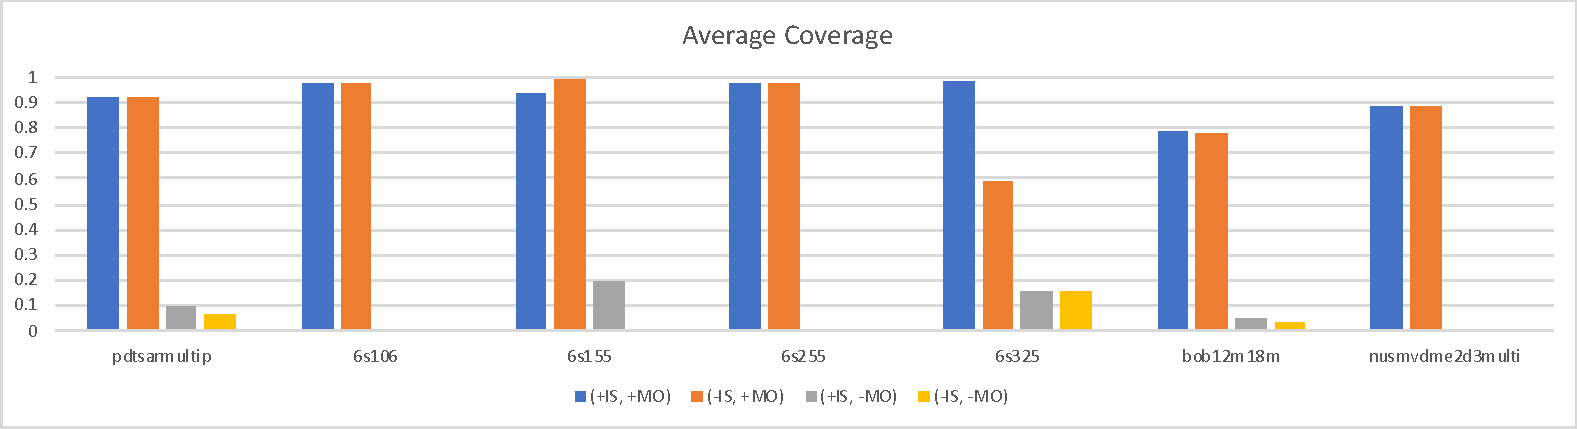
\includegraphics[width=\textwidth]{AverageCoverage}
\caption{Average requirement coverage per benchmark. A missing bar indicates a value that is approximately 0.}
\label{fig:Classification:AverageCoverage}
\vspace{0.5cm}
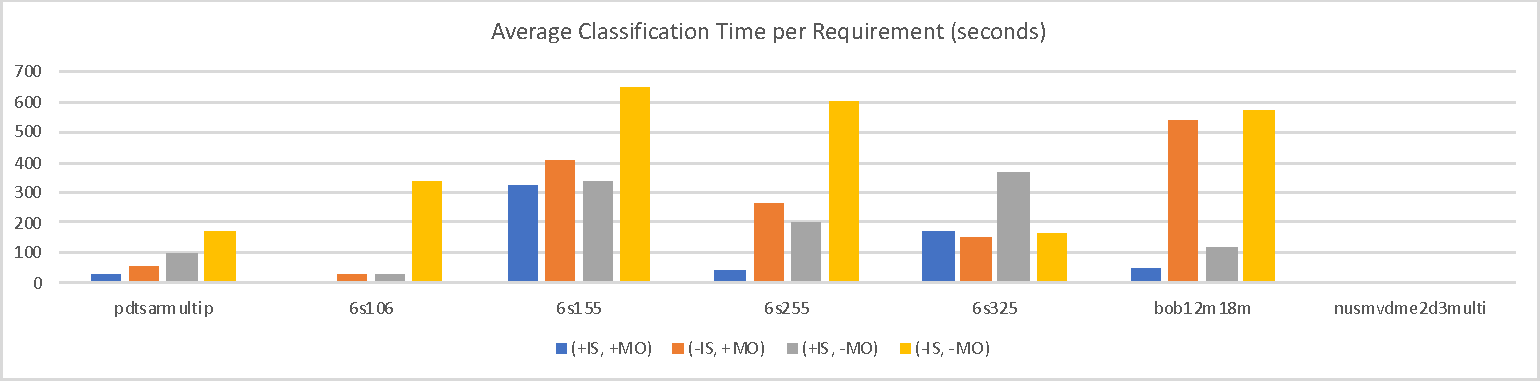
\includegraphics[width=\textwidth]{AverageExecutionTime}
\caption{Average classification time per requirement per benchmark. A missing bar indicates a value that is approximately 0. }
\label{fig:Classification:AverageExecTime}
%\end{minipage}
\end{figure}


\subsection{Partial Classification of the \texttt{pdtvsarmultip} Benchmark}
The benchmark \texttt{pdtvsarmultip} has 17 inputs, %giving values to the variables $v_{1}$ to $v_{17}$; it has 
130 latches, %ranging from $v_{18}$ to $v_{147}$; it has 
2743 gates, %ranging from $v_{148}$ to $v_{2743}$; 
and has an associated list of 33 invariant properties, out of which 31 are different (three requirements are equal). We interpret those 31 invariants as the list of security requirements. 
Since we are only considering attacker models that control latches, there are a total of $2^{130}$ attacker models that need to be classified for the 31 security requirements.
% {\color{red}

We consider six scenarios for the partial classification up to $t$ steps. We allow $t$ to take values in the set $\set{0,1,5,10,20,30}$. We obtain the execution time of classification (ms), the size of the set of source latches for the requirement (\#C), the number of minimal attacker models found (\#Min.), the total number of calls to the SAT solver (\#SAT), the average number of coordinates per minimal attacker (\#C./Min) and the coverage for the requirement (Cov.) for each requirement. We present the average of these measures in Table~\ref{tab:pdt}. 

Normally, the attacker model classification behaves in a similar way to what is reported for requirement $ \Always \lnot g_{2177}$, shown in Table~\ref{tab:pdt2324}. More precisely, coverage steadily increases and stabilises as we increase $t$. However, we like to highlight two interesting phenomena that may occur: 1) coverage {may} \emph{decrease} as we increase the time step (e.g., as shown in Table~\ref{tab:pdt2367}), and 2) the number of minimal attacker models decreases while the coverage increases, as in Tables~\ref{tab:pdt2324} and ~\ref{tab:pdt2367}. 

The coverage may decrease as we increase the time step occurs because the set of attacker models whose actions affect requirements at time 0 is rather small, i.e., $2^6$, because the effect of actions by other attackers do not have time to propagate. When we consider one step of propagation, the set of attacker models whose actions affect the requirements at times 0 and 1 has size $2^{26}$. The size of this set increases with time until it stabilises at $2^{66}$, which is the size of the set of attackers that cannot be dismissed by isolation. 

The number of minimal attacker models may decrease as the coverage increases because the minimal attacker models that are found for smaller time steps may require more components on average to break requirements than the minimal attacker models that are found when we give more time for effect of attacks to propagate. 
%represent a small percentage of the set of attackers that can affect the system, so there is very little we can learn by using monotonicity. 
More precisely, those minimal attacker models control a relatively large set of coordinates, which they need to be successful in breaking requirements, as shown in Step 5, column \#C./Min in Tables~\ref{tab:pdt2324} and~\ref{tab:pdt2367}. By considering more time steps, we are allowing attackers that control less coordinates to further propagate their actions through the system, which enables attack strategies that were unsuccessful for smaller choices of time steps.

\begin{table}[!t]
\centering
\caption{Average measures for all requirements per time steps.}
{
	%\small
\begin{tabular}{|c|c|c|c|c|c|c|}
\hline
Steps & ms &  \#C. & \#Min. & \#SAT & \#C./Min. & Cov.\\
\hline
0 & 683.12903 & 34.967741 & 2.4516129 & 16328.774 & 1.4 & 0.5272775\\
1 & 2387.5483 & 46.225806 & 6.3870967 & 24420 & 1.6502324 & 0.5725332\\
5 & 5229.9354 & 58.935483 & 44.903225 & 28355.290 & 1.6396456 & 0.849569\\
10 & 24967.129 & 58.935483 & 151.19354 & 25566.548 & 1.4608692 & 0.9189732\\
20 & 13632.516 & 58.935483 & 17.677419 & 20849.709 & 1.1762725 & 0.9793542\\
30 & 12208.258 & 58.935483 & 15.935483 & 20798.161 & 1.1045638 & 0.9793542\\
\hline
\end{tabular}}
\label{tab:pdt}
\end{table}
\begin{table}[!t]
\centering
%\begin{minipage}{0.65\textwidth}
%\begin{minipage}{0.45\textwidth}
\caption{Coverage for $\Always \lnot g_{2177}$.}
%\resizebox{\textwidth}{!}
{
\begin{tabular}{|c|c|c|c|c|c|c|}
\hline
\multicolumn{7}{|c|}{$\Always \lnot g_{2177}$} \\
\hline
Steps & ms & \#C & \#Min. & \#SAT & \#C./Min. & Cov.\\
\hline
0 & 895 & 59 & 0 & 34281 & -- & 5.94E-14\\
1 & 2187 & 66 & 10 & 47378 & 2 & 0.499511\\
5 & 1735 & 66 & 205 & 12476 & 1.912195 & 0.999997\\
10 & 968 & 66 & 27 & 9948 & 1 & 0.999999\\
20 & 1275 & 66 & 27 & 9948 & 1 & 0.999999\\
30 & 1819 & 66 & 27 & 9948 & 1 & 0.999999\\
 \hline
\end{tabular}
}
\label{tab:pdt2324}
\end{table}

% \end{minipage}
% \vspace{1cm}
% \begin{minipage}{0.45\textwidth}
\begin{table}[!t]
	\centering
\caption{Coverage for $\Always \lnot g_{2220}$.}
%\resizebox{\textwidth}{!}
{
\begin{tabular}{|c|c|c|c|c|c|c|}
\hline
\multicolumn{7}{|c|}{$\Always \lnot g_{2220}$} \\
\hline
Steps & ms &  \#C. & \#Min. & \#SAT & \#C./Min. & Cov.\\
\hline
0 & 1 & 6 & 1 & 28 & 1 & 0.90625\\
1 & 86 & 26 & 1 & 2628 & 1 & 0.500039\\
5 & 4511 & 67 & 17 & 47664 & 2.588235 & 0.852539\\
10 & 3226 & 67 & 6 & 37889 & 1 & 0.984375\\
20 & 3355 & 67 & 6 & 37889 & 1 & 0.984375\\
30 & 3562 & 67 & 6 & 37889 & 1 & 0.984375\\
 \hline
\end{tabular}
}
\label{tab:pdt2367}
% \end{minipage}
\end{table}


By taking an average over all requirements, we observe that coverage seems to steadily increase as we increase the number of steps for the classification, as reported in Table~\ref{tab:pdt}, column Cov. The low coverage for small $t$ is due to the restriction on the size of minimal attacker models; if we allowed more coordinates for minimal attackers, then the effect of their attacks may propagate faster to the target requirements. More precisely, for small $t$, attackers can only use short strategies, which limits their interaction with the system. In this sense, we expect minimal attacker models to control a large number of coordinates if they want to successfully influence a requirement in a single time step, and since we restricted our search to attacker models of maximum size three, those larger attacker models remain unexplored (e.g., as reported in Table~\ref{tab:pdt2324} for Step 0).

We conclude that experimental evidence favours the use of both monotonicity and isolation for the classification of attacker models, although some exceptions may occur for the use of isolation. In general, monotonicity and isolation help the classification methodology $(+IS,+MO)$ consistently obtain significantly better coverage compared to the naive methodology $(-IS,-MO)$.
%-------------------------------------------------------------------------------------------------------------------------------------------------

\section{Related Work}
\label{sec:discussion}
\paragraph{On Defining Attackers.} Describing an adequate attacker model to contextualise the security guarantees of a system is not a trivial task. Some attacker models may be adequate to provide guarantees over one property, but not for a different one (e.g., the Dolev-Yao attacker model is sensible for confidentiality properties, but not so much for integrity properties). Additionally, depending on the nature of the system and the security properties being studied, it is sensible to describe attackers at different levels of abstraction. For instance, in the case of security protocols, Basin and Cremers define attackers in~\cite{KnowYourEnemy} as combinations of compromise rules that span over three dimensions:  \emph{whose} data is compromised, \emph{which} kind of data it is, and \emph{when} the compromise occurs. In the case of Cyber-physical Systems (CPS), works like \cite{Giraldo2018} model attackers as sets of components (e.g., some sensors or  actuators), while other works like \cite{IFCPSSec,Cardenas2011,Urbina2016} model attackers that can arbitrarily manipulate any control inputs and any sensor measurements at will, as long as they avoid detection. In the same context of CPS, Rocchetto and Tippenhauer \cite{CPSProfiles} model attackers more abstractly as combinations of quantifiable traits (e.g., insider knowledge, access to tools, and financial support); these traits, when provided a compatible system model, ideally fully define how the attacker can interact with the system. 


Our methodology for the definition of attackers combines aspects from~\cite{KnowYourEnemy} and \cite{Giraldo2018}. The authors of~\cite{KnowYourEnemy} define symbolic attackers and a set of rules that describe how the attackers affect the system, which is sensible since many cryptographic protocols are described symbolically. Our methodology describes attackers as sets of coordinates (staying closer to the definitions of attackers in \cite{Giraldo2018}), and has a lower level of abstraction since we describe the semantics of attacker actions in terms of how they change the functional behaviour of the AIG, and not in terms of what they ultimately represent. This lower level of abstraction lets us systematically and exhaustively generate attacker models for a given system by using the definition of such system, but those models do not automatically translate to other systems. Basin and Cremers compare the effect of attackers across different protocol implementations because their attacker models have the same abstract semantics. If we had an abstraction function from sets of gates and latches to abstract effects (e.g., ``gates in charge of encryption'', or ``latches in charge of redundancy''), then it could be possible to compare results amongst different AIGs.

In Chapter~\ref{ch:CPSRobustness}, we expand the notion of attacker models that we used in this chapter, i.e., attacker models as sets of coordinates, by adding a new component: \emph{attack preconditions}. If coordinates determine \emph{which} components are compromised and \emph{how}, then attack preconditions define \emph{when} they are compromised.

\paragraph{On Efficient Classification.} 
The works by Cabodi, Camurati and Quer \cite{GraphLabelingForEfficientCOIComputation}, Cabodi et. al \cite{ToSplitOrToGroup}, and Cabodi and Nocco \cite{OptimizedModelCheckingOfMultipleProperties} present several useful techniques that may improve the performance of model checking when verifying multiple properties, including COI reduction and property clustering. We also mention the work by Goldberg et al. \cite{JustAssume} where they consider the problem of efficiently checking a set of safety properties $P_1$ to $P_k$ by individually checking each property while assuming that all other properties are valid. These works inspired us to incrementally check requirements in the same cluster, helping us transform Equation~\ref{eq:naiveCheck} into Equation~\ref{eq:MasterEq}. Nevertheless, we note that all these techniques are described for model checking systems in the absence of attackers, which is why we needed to introduce the notions of isolation and monotonicity to account for them. We believe that it may be possible to use or incorporate other techniques that improve the efficiency of BMC in general (e.g., interpolation \cite{Interpolation}), but such optimisations are beyond the scope of this work.

\paragraph{On Completeness.} As mentioned in Section~\ref{sec:completeness}, if the time parameter for the classification is below the {completeness threshold}, the resulting attacker model classification is most likely {incomplete}. To guarantee completeness, it may be possible to adapt existing termination methods (e.g. \cite{ProvingMorePropertiesWithBMC}) to incorporate attacker models. Alternatively, methods that compute a good approximation of the completeness threshold (e.g. \cite{EfficientComputationOfRecurrenceDiameters}) should not only improve coverage in general but also the reliability of the resulting attacker model classifications.  Interpolation \cite{Interpolation} could also help finding a guarantee of completeness. 

Finally, if we consider alternative verification techniques to BMC, then IC3 \cite{IC3,IC32} and PDR \cite{IC3}, which have seen some success in hardware model checking, may address the limitation of boundedness.

\paragraph{On Verifying Non-Safety Properties.} In this work, we focused our analysis exclusively on safety properties of the form $\Always e$. However, it is possible to extend this methodology to other types of properties, as it is possible to efficiently encode Linear Temporal Logic formulae for bounded model checking \cite{BMCWithoutBDDs,lmcs:2236}. The formulations of the SAT problem change for the different formulae, but both isolation and monotonicity should remain valid heuristics; ultimately, monotonicity and isolation are about the sound extrapolation of the validity of attack strategies among attacker models that have related capabilities.

\section{Summary and Conclusion}
\label{sec:Classification:Summary}
In this chapter, we model AIGs as $F$-coalgebras, and we model their attackers using sets of spatial transformations. We use bounded model checking to classify and compare attackers, which provides an answer for Research Question~\ref{que:Classification} in the case of AIGs. Due to the exponential size of the problem, we propose a set of heuristics to perform bounded model-checking efficiently, for which we provide experimental evidence. 


% In this chapter, we presented a methodology to model check systems in the presence of attackers with the objective of mapping each attacker model to the set of security requirements broken by attackers that fit the model. This mapping of attacker models creates a classification for them, defining equivalence classes of attacker models by both set inclusion and by the set of requirements broken by their attackers. While it is possible to perform a classification of attackers by exhaustively performing model checking, the exponential size of the set of attackers renders a naive approach impractical. Thus, we rely on ordering relations between attackers to efficiently classify a large percentage of them. We provide empirical evidence by applying our methodology to a set of AIG benchmarks, which describe hardware systems at a bit level.
Finding minimal attacker models with only one coordinate is relatively simple since AIGs are systems where a fault quickly propagates through the system. Informally, this means that the systems we studied were not very robust: all it takes is for one of several components to fail or be attacked to cause these systems to fail their security requirements. Since altering a single component already causes systems to fail, we conclude that using SAT solvers and BMC was excessive for attacker classification; it could have sufficed to test systematically the systems instead of checking them. Consequently, we switch from verification to testing in Chapter~\ref{ch:CPSRobustness}. 

% The contents of this chapter are published in ~\cite{SystematicClassification}.

% and they can give us attacks, but that maybe we need not verify a system: we should test them instead, since we expect them to fail when in the presence of attackers. This takes us to the second application on CPSs

% A system is considered safe in the presence of attackers if no attacker model breaks any requirement. However, In our view, ensuring the completeness of the attacker model classification is the most relevant direction for future work. Unlike complete classifications, incomplete classifications cannot provide guarantees that work in the general case if minimal attackers are not found. We also note that the effectiveness of monotonicity for classification is directly related to finding minimal attackers. Consequently, our methodology may benefit from any other method that helps in the identification of those minimal attackers. In particular, we are interested in checking the effectiveness of an approach where, instead of empowering attackers, we try to {reduce} successful attackers into minimal attackers by removing unnecessary capabilities. This, formally, is an \emph{actual causality analysis} \cite{ActualCausality} of successful attackers.

%-------------------------------------------------------------------------------------------------------------------------------------------------

\newpage
\begin{landscape}
	\begin{table}[!t]
		\centering		
		\centering
		\begin{tabular}{|c|c|c|c|c|c|c|c|}
			\hline
			Benchmark  & pdtsarmultip & 6s106       & 6s155       & 6s255       & 6s325       & bob12m18m   & nusmvdme2d3multi \\ \hline
			\multicolumn{8}{|c|}{Average Coverage per Requirement}                                                             \\ \hline
			(+IS, +MO) & 0.918973269  & 0.977620187 & 0.93762207  & 0.977172852 & 0.986949581 & 0.785075777 & 0.8853302        \\
			(-IS, +MO) & 0.916622423  & 0.977008259 & 0.99609375  & 0.9765625   & 0.590205544 & 0.781704492 & 0.8853302        \\
			(+IS, -MO) & 9.95E-02     & 2.01E-03    & 0.1953125   & 1.73828E-11 & 0.156147674 & 4.61E-02    & 4.52E-15         \\
			(-IS, -MO) & 6.45E-02     & 9.10E-36    & 6.00E-72    & 2.0838E-222 & 0.156146179 & 3.29E-02    & 4.52E-15         \\ \hline
			\multicolumn{8}{|c|}{Average Classification Time per Requirement}                                                  \\ \hline
			(+IS, +MO) & 24967.12903  & 3088.882353 & 326372.2188 & 38396.125   & 174066.6047 & 49916.59211 & 3530.666667      \\
			(-IS, +MO) & 56187.48387  & 25090.47059 & 408165.4063 & 263457.125  & 152425.3889 & 541870.25   & 3348.333333      \\
			(+IS, -MO) & 97326.29032  & 28483.11765 & 340715.0313 & 197275.75   & 363913.8472 & 114330.0855 & 3890             \\
			(-IS, -MO) & 170630.7742  & 341430.7059 & 646926.0625 & 602012.5    & 162959.5436 & 572080.0987 & 4262.333333      \\ \hline
			\multicolumn{8}{|c|}{Average Number of Components to Build Attackers From per Requirement}                         \\ 
			\hline
			(+IS, +MO) & 58.93548387  & 35.47058824 & 9           & 93.875      & 173.1196013 & 124.0460526 & 63               \\
			(-IS, +MO) & 82           & 135         & 257         & 752         & 1668        & 261         & 63               \\
			(+IS, -MO) & 58.93548387  & 35.47058824 & 9           & 93.875      & 173.1196013 & 124.0460526 & 63               \\
			(-IS, -MO) & 82           & 135         & 257         & 752         & 1668        & 261         & 63               \\ 
			\hline
			% \multicolumn{8}{|c|}{Average Number of Identified Successful Attackers per Requirement}                            \\ \hline
			% (+IS, +MO) & 151.1935484  & 16.05882353 & 7.5         & 2.5625      & 237.3056478 & 34.93421053 & 129.3333333      \\
			% (-IS, +MO) & 146.0322581  & 16.05882353 & 8           & 2.4375      & 46.42424242 & 34.68421053 & 129.3333333      \\
			% (+IS, -MO) & 15860.25806  & 14693.17647 & 98          & 13792.9375  & 214293.01   & 22700.58553 & 1282             \\
			% (-IS, -MO) & 27207.54839  & 105842.7059 & 126133.2813 & 20657       & 2502.25641  & 40526.72368 & 1282             \\ 
			% \hline
			% \multicolumn{8}{|c|}{Average Number of Calls to SAT Solver per Requirement}                                        \\ \hline
			% (+IS, +MO) & 25566.54839  & 1978.647059 & 10.4375     & 11382.125   & 583123.7209 & 300825.9605 & 40576.33333      \\
			% (-IS, +MO) & 58420.83871  & 294477.9412 & 2022640.25  & 35252.1875  & 51411.24747 & 1607803.138 & 40576.33333      \\
			% (+IS, -MO) & 41275.6129   & 16655.76471 & 101         & 23455.875   & 550652.3721 & 322031.1513 & 41729            \\
			% (-IS, -MO) & 85390.80645  & 396510      & 1389339.563 & 49366.1875  & 56238.01026 & 1266308.526 & 41729            \\ \hline
			% \multicolumn{8}{|c|}{Average Minimal Number of Components Needed by Successful Attackers per Requirement}          \\ 
			% \hline
			% (+IS, +MO) & 1.460869285  & 1.004524887 & 1           & 0.464285714 & 1.649279888 & 1.142237928 & 2.843533741      \\
			% (-IS, +MO) & 1.460869285  & 1.004524887 & 1           & 0.4375      & 1           & 1.123402209 & 2.843533741      \\
			% (+IS, -MO) & 2.912532493  & 2.909934933 & 2.1953125   & 2.885495873 & 2.927835684 & 2.964760733 & 2.984195449      \\
			% (-IS, -MO) & 2.975171828  & 2.983304749 & 2.665659086 & 1.986925862 & 1.977314997 & 2.973301799 & 2.984195449      \\ \hline
	\end{tabular}
		\caption{Average metrics per requirement for the different benchmarks (Continued in Figure~\ref{tab:Classification:AllResults2})}
		\label{tab:Classification:AllResults1}
		\end{table}	
\end{landscape} 
\newpage
\begin{landscape}
	\begin{table}[!t]
		\centering		
		\centering
		\begin{tabular}{|c|c|c|c|c|c|c|c|}
			\hline
			Benchmark  & pdtsarmultip & 6s106       & 6s155       & 6s255       & 6s325       & bob12m18m   & nusmvdme2d3multi \\ \hline
			% \multicolumn{8}{|c|}{Average Coverage per Requirement}                                                             \\ \hline
			% (+IS, +MO) & 0.918973269  & 0.977620187 & 0.93762207  & 0.977172852 & 0.986949581 & 0.785075777 & 0.8853302        \\
			% (-IS, +MO) & 0.916622423  & 0.977008259 & 0.99609375  & 0.9765625   & 0.590205544 & 0.781704492 & 0.8853302        \\
			% (+IS, -MO) & 9.95E-02     & 2.01E-03    & 0.1953125   & 1.73828E-11 & 0.156147674 & 4.61E-02    & 4.52E-15         \\
			% (-IS, -MO) & 6.45E-02     & 9.10E-36    & 6.00E-72    & 2.0838E-222 & 0.156146179 & 3.29E-02    & 4.52E-15         \\ \hline
			% \multicolumn{8}{|c|}{Average Classification Time per Requirement}                                                  \\ \hline
			% (+IS, +MO) & 24967.12903  & 3088.882353 & 326372.2188 & 38396.125   & 174066.6047 & 49916.59211 & 3530.666667      \\
			% (-IS, +MO) & 56187.48387  & 25090.47059 & 408165.4063 & 263457.125  & 152425.3889 & 541870.25   & 3348.333333      \\
			% (+IS, -MO) & 97326.29032  & 28483.11765 & 340715.0313 & 197275.75   & 363913.8472 & 114330.0855 & 3890             \\
			% (-IS, -MO) & 170630.7742  & 341430.7059 & 646926.0625 & 602012.5    & 162959.5436 & 572080.0987 & 4262.333333      \\ \hline
			% \multicolumn{8}{|c|}{Average Number of Components to Build Attackers From per Requirement}                         \\ 
			% \hline
			% (+IS, +MO) & 58.93548387  & 35.47058824 & 9           & 93.875      & 173.1196013 & 124.0460526 & 63               \\
			% (-IS, +MO) & 82           & 135         & 257         & 752         & 1668        & 261         & 63               \\
			% (+IS, -MO) & 58.93548387  & 35.47058824 & 9           & 93.875      & 173.1196013 & 124.0460526 & 63               \\
			% (-IS, -MO) & 82           & 135         & 257         & 752         & 1668        & 261         & 63               \\ 
			% \hline
			\multicolumn{8}{|c|}{Average Number of Identified Successful Attackers per Requirement}                            \\ \hline
			(+IS, +MO) & 151.1935484  & 16.05882353 & 7.5         & 2.5625      & 237.3056478 & 34.93421053 & 129.3333333      \\
			(-IS, +MO) & 146.0322581  & 16.05882353 & 8           & 2.4375      & 46.42424242 & 34.68421053 & 129.3333333      \\
			(+IS, -MO) & 15860.25806  & 14693.17647 & 98          & 13792.9375  & 214293.01   & 22700.58553 & 1282             \\
			(-IS, -MO) & 27207.54839  & 105842.7059 & 126133.2813 & 20657       & 2502.25641  & 40526.72368 & 1282             \\ 
			\hline
			\multicolumn{8}{|c|}{Average Number of Calls to SAT Solver per Requirement}                                        \\ \hline
			(+IS, +MO) & 25566.54839  & 1978.647059 & 10.4375     & 11382.125   & 583123.7209 & 300825.9605 & 40576.33333      \\
			(-IS, +MO) & 58420.83871  & 294477.9412 & 2022640.25  & 35252.1875  & 51411.24747 & 1607803.138 & 40576.33333      \\
			(+IS, -MO) & 41275.6129   & 16655.76471 & 101         & 23455.875   & 550652.3721 & 322031.1513 & 41729            \\
			(-IS, -MO) & 85390.80645  & 396510      & 1389339.563 & 49366.1875  & 56238.01026 & 1266308.526 & 41729            \\ \hline
			\multicolumn{8}{|c|}{Average Minimal Number of Components Needed by Successful Attackers per Requirement}          \\ 
			\hline
			(+IS, +MO) & 1.460869285  & 1.004524887 & 1           & 0.464285714 & 1.649279888 & 1.142237928 & 2.843533741      \\
			(-IS, +MO) & 1.460869285  & 1.004524887 & 1           & 0.4375      & 1           & 1.123402209 & 2.843533741      \\
			(+IS, -MO) & 2.912532493  & 2.909934933 & 2.1953125   & 2.885495873 & 2.927835684 & 2.964760733 & 2.984195449      \\
			(-IS, -MO) & 2.975171828  & 2.983304749 & 2.665659086 & 1.986925862 & 1.977314997 & 2.973301799 & 2.984195449      \\ \hline
	\end{tabular}
		\caption{Average metrics per requirement for the different benchmarks (Cont. of Figure~\ref{tab:Classification:AllResults1})}
		\label{tab:Classification:AllResults2}
		\end{table}	
\end{landscape} 